\chapter{Implementation and discussion} \label{chap: Result}

In order to verify the feasibility of the methodologies from chapter \ref{chap: Meth}, 
performance testing based on assumptions and two industrial uses cases 
are done and their results will be performed and discussed in this chapter. 
Again, the tests will also be divided into internal (\ref{chap: Result-Internal}) 
and external (\ref{chap: Result-External}) part, referring to those in chapter \ref{chap: Meth}.

\section{Internal}\label{chap: Result-Internal}
For the internal \gls{mas}, multiple tests are performed on the agent 
communication system. That means, the messages 
will be passed through the \gls{ca} under WebSocket architecture. 
Various tests will be done and the test results will be discussed later in section 
\ref{chap: Result-WS}. 
In addition to the performance testing of WebSocket architecture alone, 
a comparison between WebSocket and RestFUL API will be done to verify the feasibility 
of WebSocket. 
Finally, tests relevant to packets prioritization will be performed to close 
the sections. 


\subsection{Test results of WebSocket in various performance testing including worst case scenarios} \label{chap: Result-WS}

After the construction a \gls{mas} under WebSocket, the speed, robustness, 
reliability and application size of the system will be examined by 
performance tests. 

\subsubsection{Increasing client numbers}
In real world, the number of clients will greatly influence the performance of 
server. Assume that all agents serve as clients and \gls{ca} as a central server. 
  

By handling an increasing number of connection requests, and the growing demands 
of data processing capacity, the average total delay with or without process time can be 
roughly described as an overall increasing pattern. However, it does not necessarily 
need to be linear based on several reasons. In exercise, concurrent programming 
will speed up the processing for a large computation problem. As depicted in 
fig.\ref{fig: proportional-clients}, the average process time from one to ten 
clients is decreasing with a better utilization of the CPU power due to 
concurrent processing. However, by further increasing the clients number, the 
speedup will be limited by CPU cores number. Assume that a CPU has 8 core, 
and each core can handle 2 threads, it will have in total 16 threads to perform tasks.
In WebSocket based \gls{mas} program, the asynchronous I/O framework asyncio is used 
to handle the coroutines execution in order to better utilize the threads power.
Therefore, the asyncio is potentially more suitable for larger computational tasks 
compared to synchronous single thread programming.

Obviously there is a limit of the clients number to prevent system breakdown. 
With one server handling all clients at once, there is a system timeout problem of 
the server when the clients number reaches 1000. Therefore, 
distributing clients with more servers becomes a possible solution. 


\begin{figure}[htb]
    \begin{subfigure}[b]{0.49\textwidth}
        \centering
        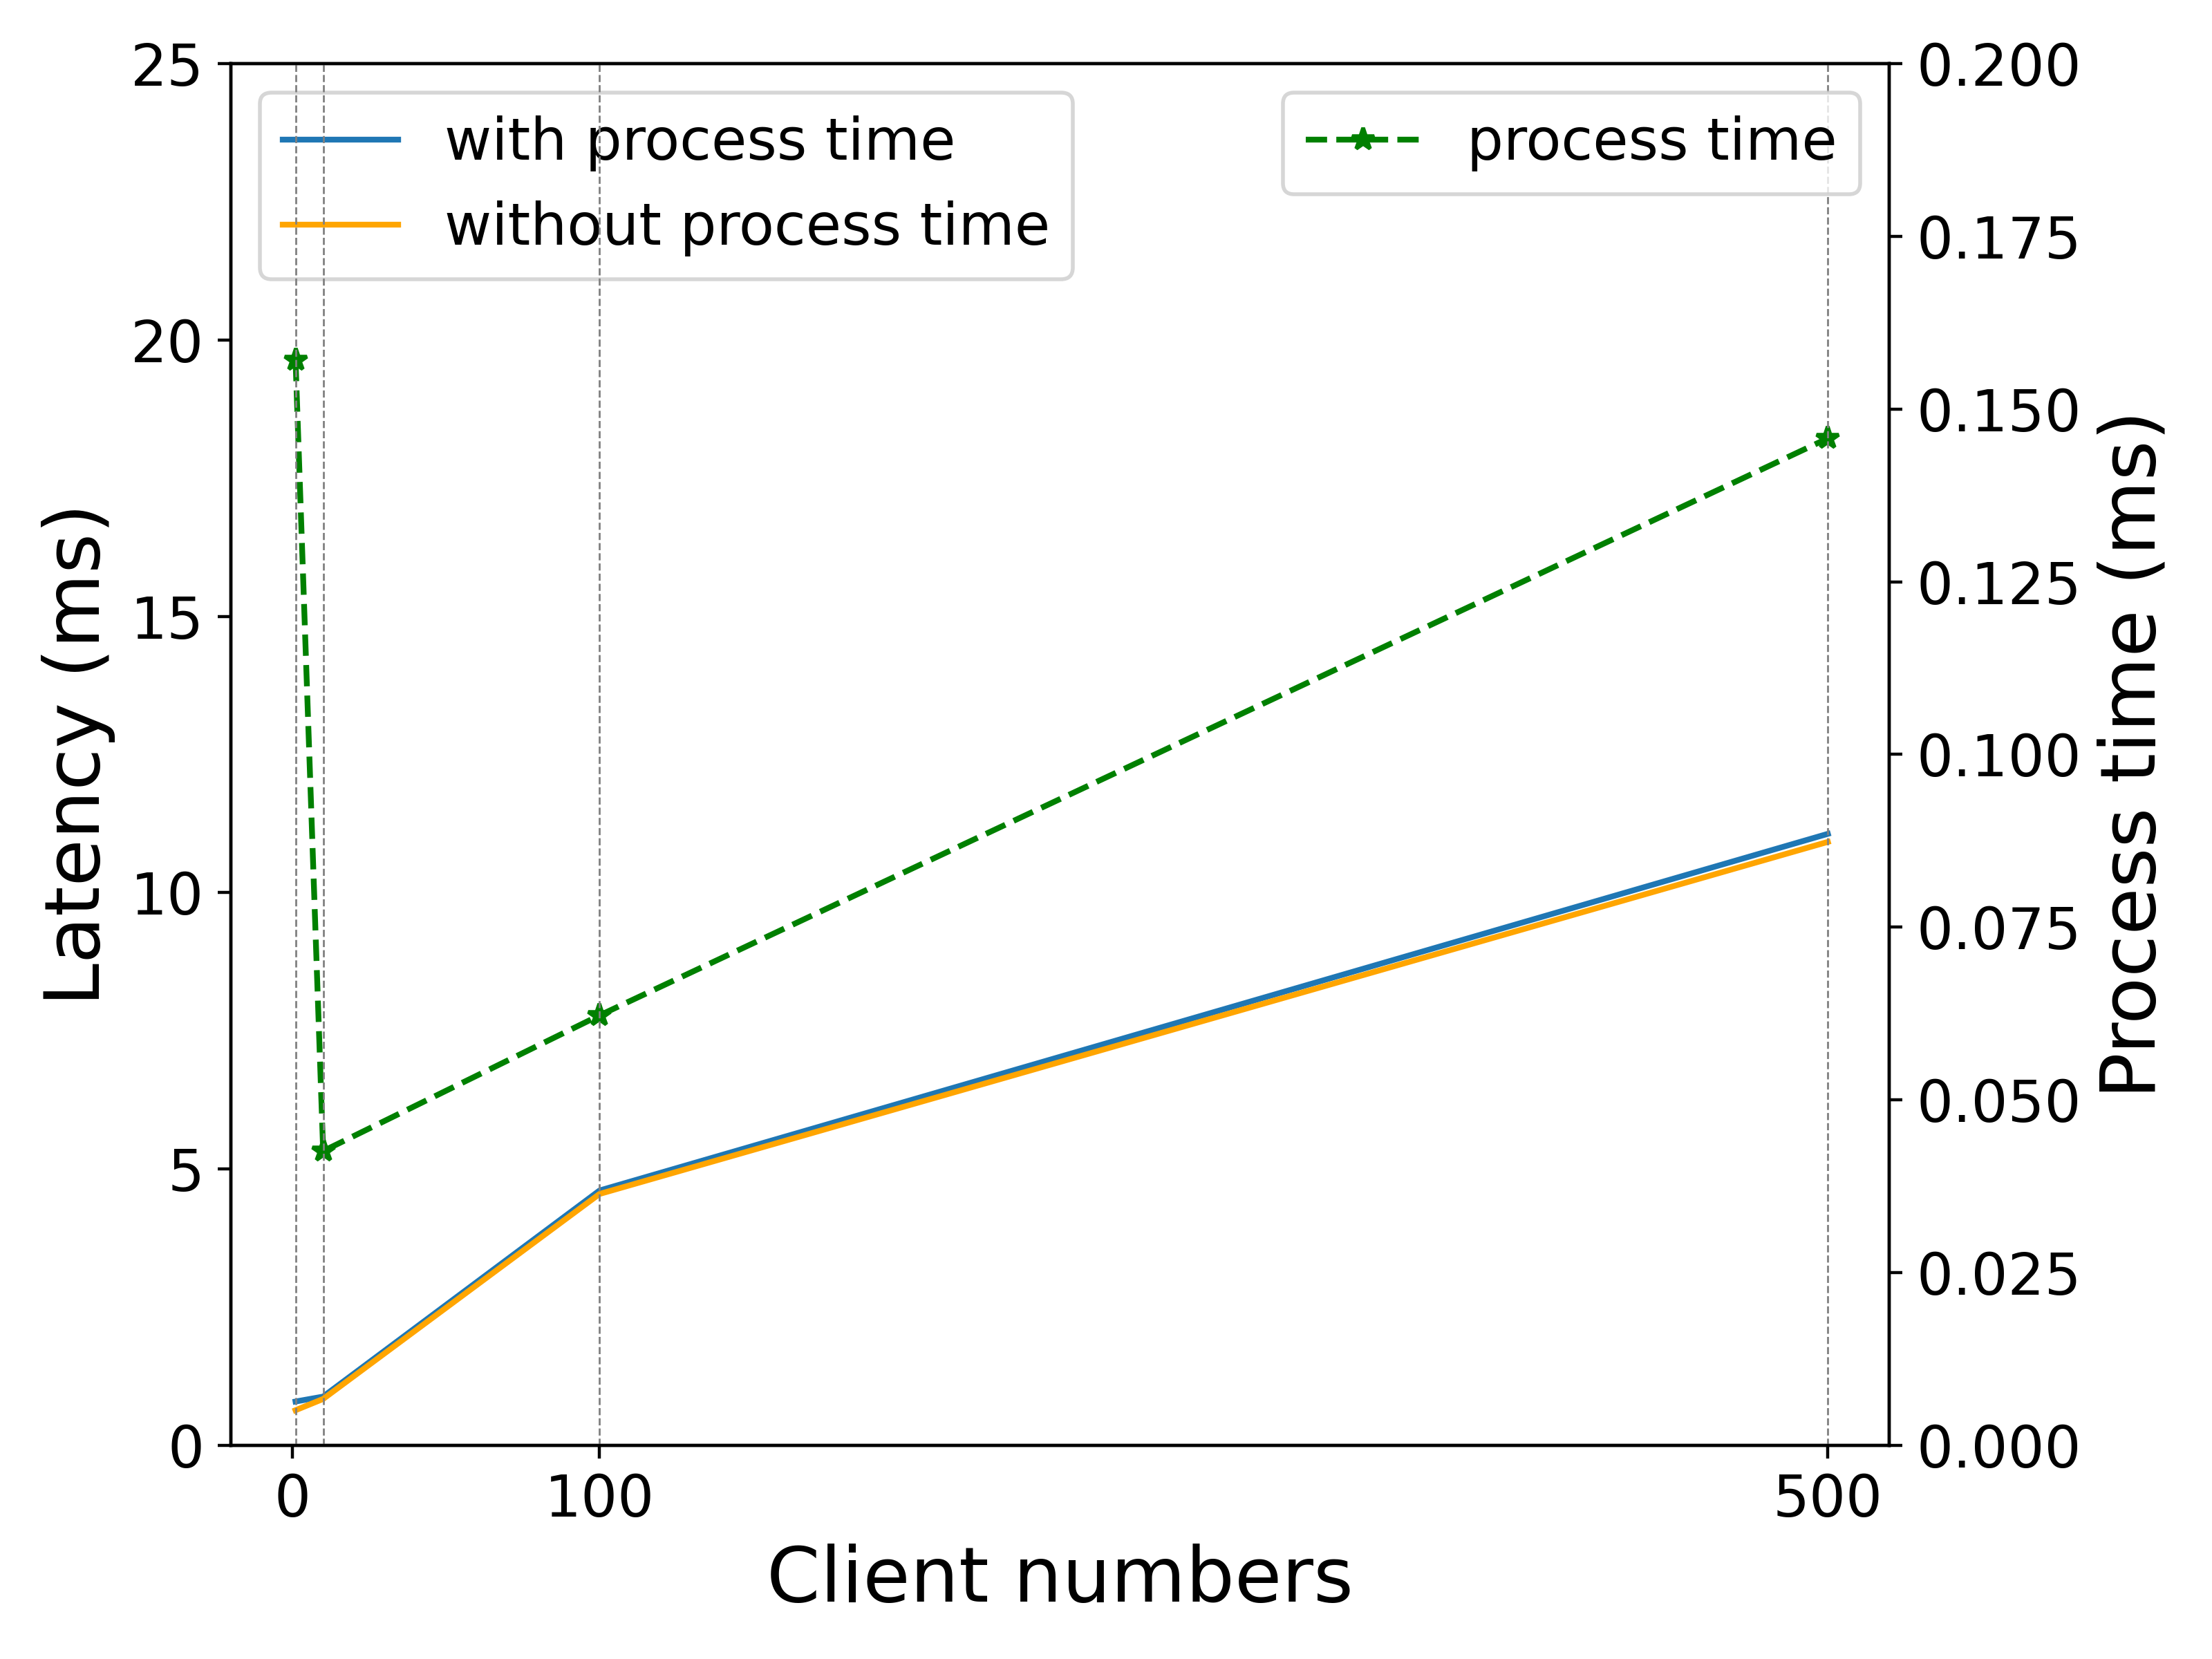
\includegraphics[width=\textwidth]{figures/tests/proportional_tests/Average_string_messages_sending_time_of_100_tests_of_diff_client_numbers.png}\hfill 
        \caption{} \label{fig: proportional-clients-a}
    \end{subfigure}
    \begin{subfigure}[b]{0.49\textwidth}
        \centering
        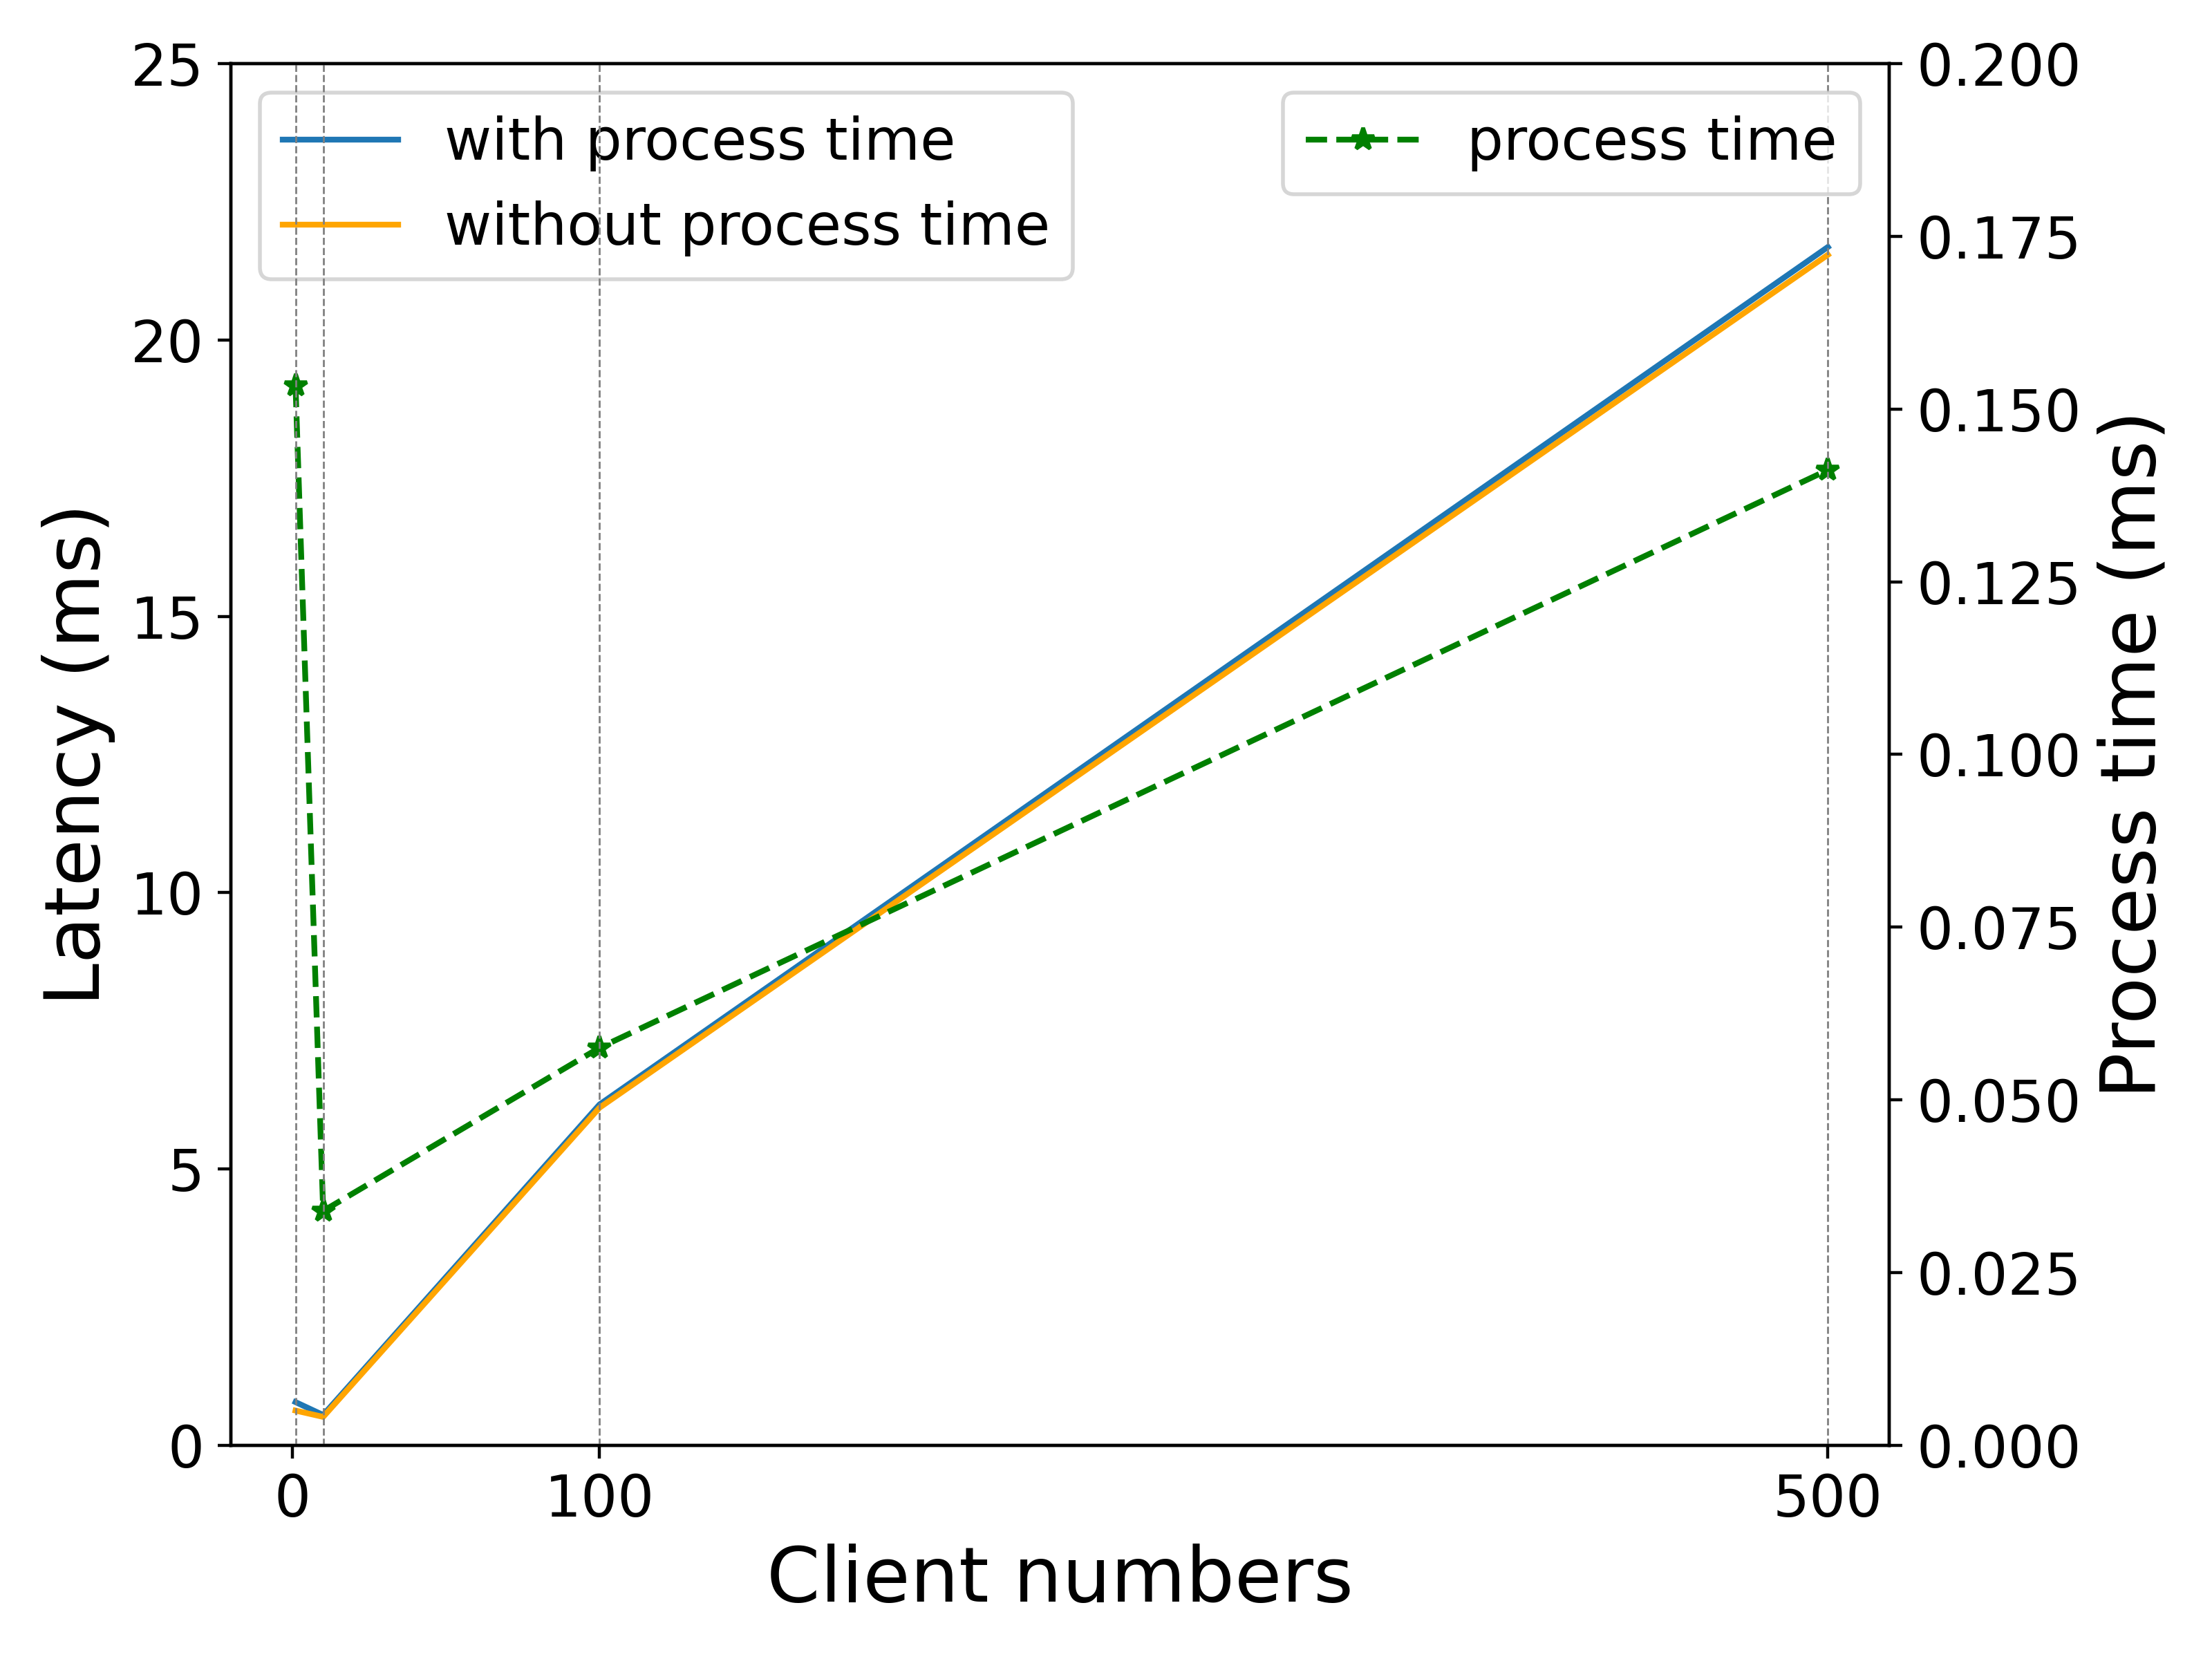
\includegraphics[width=\textwidth]{figures/tests/proportional_tests/Average_string_messages_receiving_time_of_100_tests_of_diff_client_numbers.png}\hfill 
        \caption{} \label{fig: proportional-clients-b}
        \end{subfigure}

    \caption{Average delay of sending a string message 100 times 
    to a clientR from 1, 10, 100 or 500 clients separately. (a) Messages sent forward, 
    and (b) response messages from clientR. 
    \label{fig: proportional-clients}}
\end{figure}


\subsubsection{Increasing server numbers}
Under the same condition where 1000 clients are sending and receiving messages from 
a clientR, the messages will be separated this time to two or three groups, with 
each passing through different servers. Limited by the hardware configuration 
for the external routing solutions according to fig.\ref{fig: NSConceptual}, only 
maximal three servers can be used for the test. However, several assumptions 
can be made based on the results from fig.\ref{fig: proportional-servers}. 


\begin{figure}[htb]
    \centering
    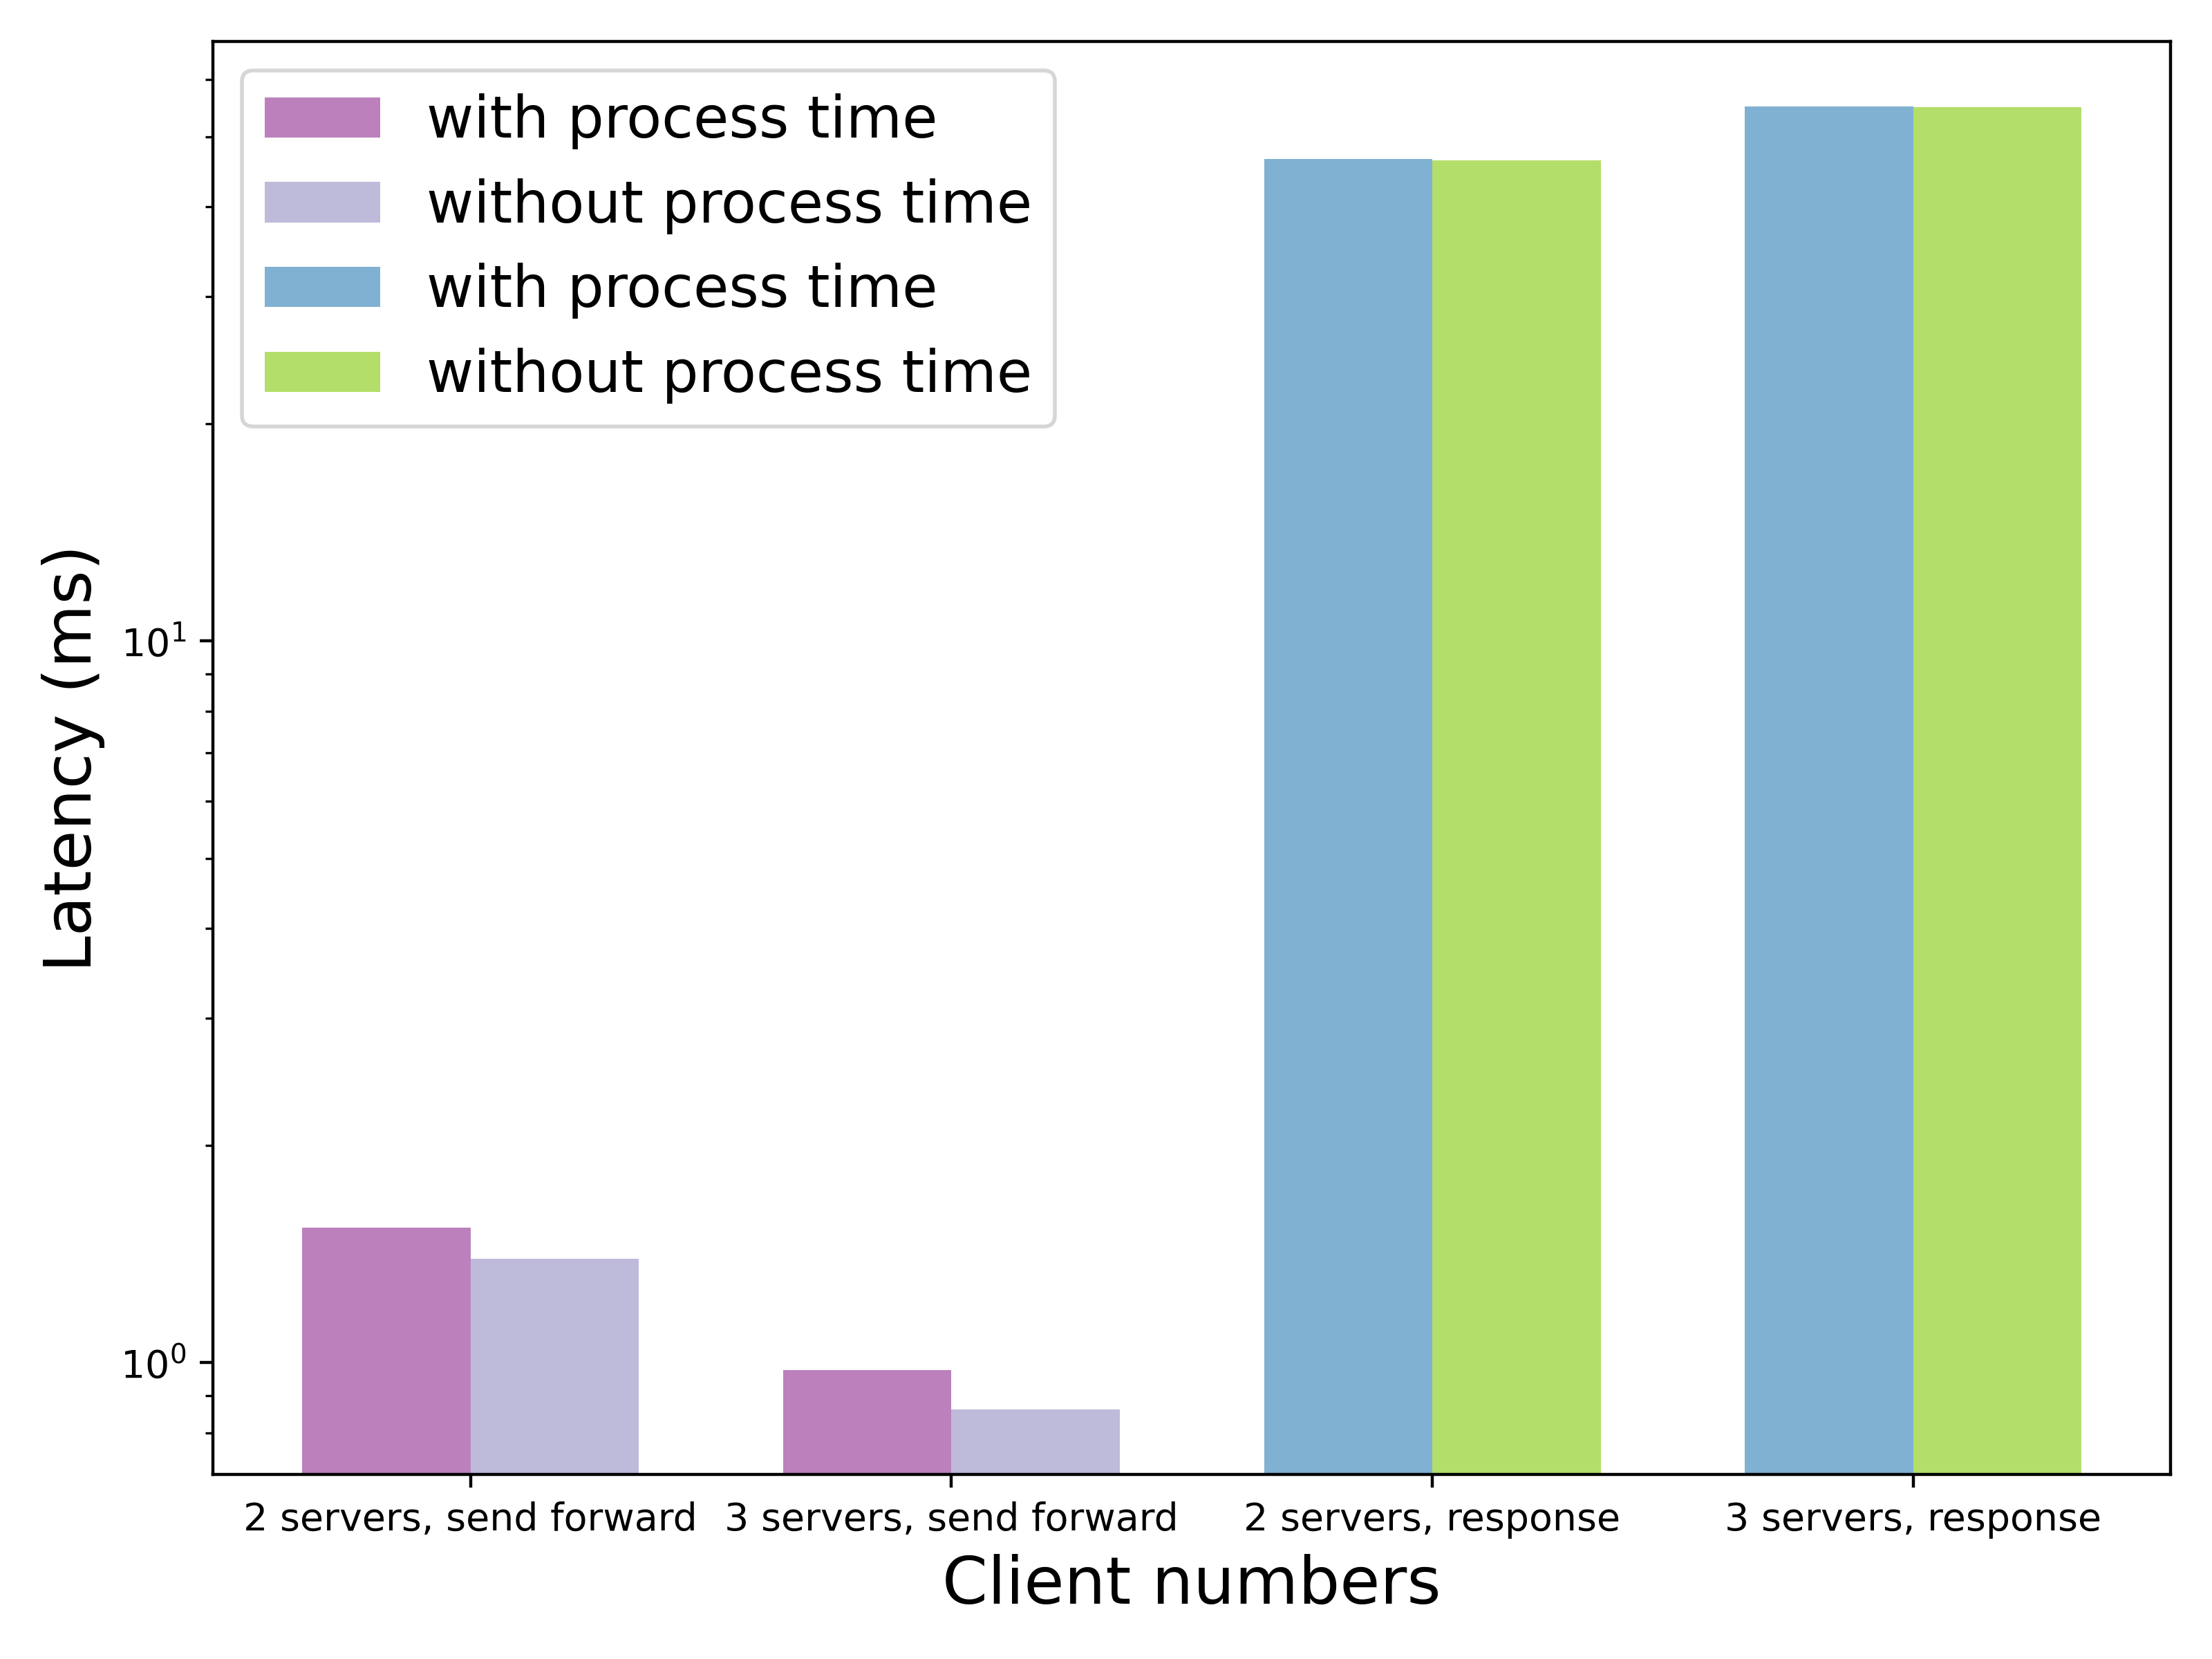
\includegraphics[width=0.8\textwidth]{figures/tests/proportional_tests/Average_string_messages_receiving_time_of_100_tests_diff_server_numbers.png}\hfill 
    \caption{Average delay of sending a string message 100 times 
    to a clientR from 1000 clients through 2 or 3 servers separately. 
    \label{fig: proportional-servers}}
\end{figure}

The latency reduction with an additional server according to 
fig.\ref{fig: proportional-servers} proves that, by introducing more servers 
to the system, the limited productive resources should be better utilized 
for frequent clients interactions. However, not as expected, the latency of 
response messages from clientR is much larger in fig.\ref{fig: proportional-servers},
which may also result from the CPU consumption. Since the send and receive 
processes in websocket are operated separately, and because of the high 
occupation of the CPU power when more than one server are running in the same 
device, the loads between each process might be unbalanced and added up by the 
increment of servers. 


\subsubsection{Increasing string message length}
Another important test should be done to verify the influence of packet size (i.e., 
message length) to the system performance, according to the formula of packet 
transmission time: 
\begin{equation}
    Transmission $ $ delay = Packet $ $ size/Bandwidth
\end{equation}

If the bandwidth is determined, the transmission time with an increasing packet 
size should be linear. In the fig.\ref{fig: proportional-stringsize}, comparisons 
between different string message lengths varied from 1KB to 10MB are examined. 
The linear dependency of latency and string size in both forward 
(fig.\ref{fig: proportional-stringsize-a}) and return message (fig.\ref{fig: proportional-stringsize-b}) 
has verified the transmission time formula. It is also noticeable that the server 
process time increases by the rising message byte number. In real world scenarios, 
a large string message should be chunked into smaller pieces for communication, 
which will significantly reduce the process time. For the purpose of system limit 
inspection, a string with the size up to 100MB is also tested and resulting in 
system timeout error, which already exceeds the server maximal 
processing capacity. 


\begin{figure}[htb]
    \begin{subfigure}{0.49\textwidth}
        \centering
        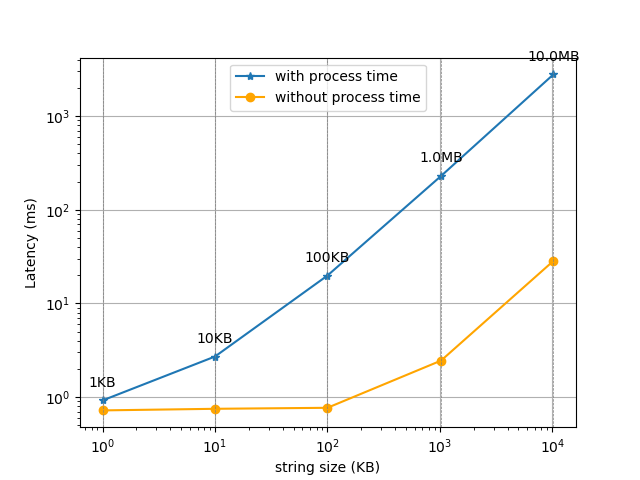
\includegraphics[width=\textwidth]{figures/tests/proportional_tests/log_Average_string_messages_sending_time_of_100_tests_1KB_to_10MB.png}
        \caption{} \label{fig: proportional-stringsize-c}
    \end{subfigure}
    \begin{subfigure}{0.49\textwidth}
        \centering
        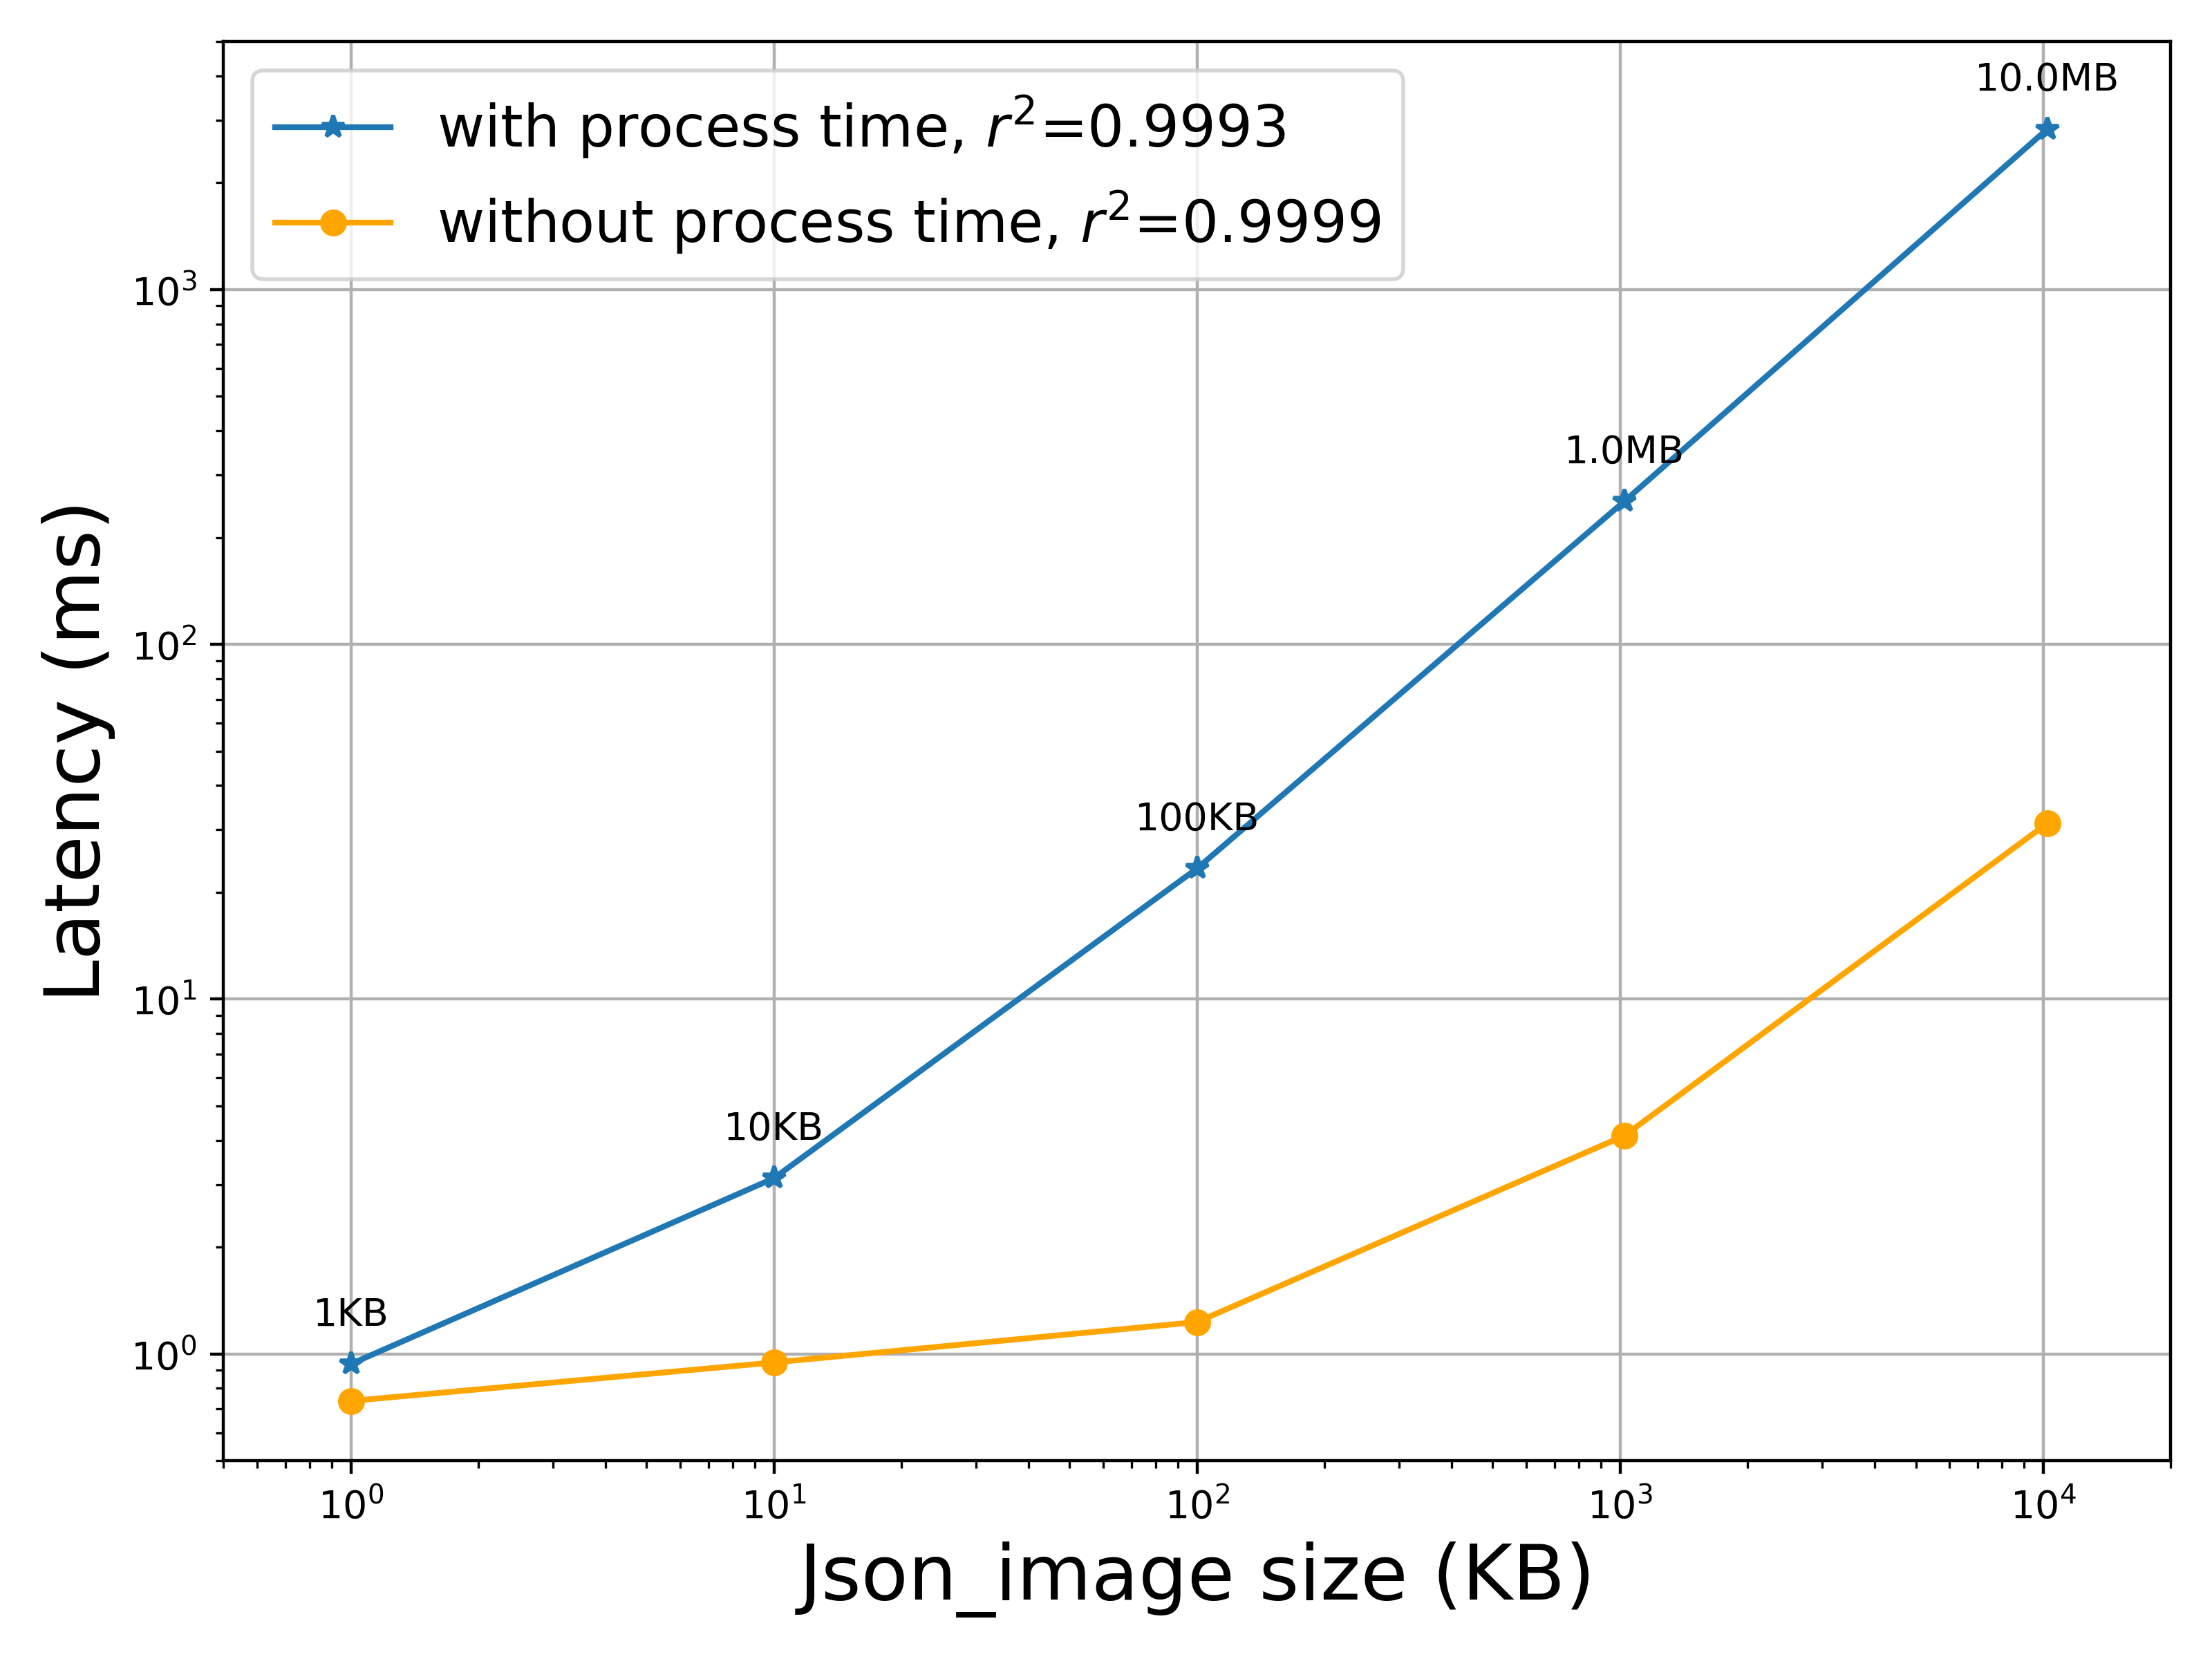
\includegraphics[width=\textwidth]{figures/tests/proportional_tests/log_Average_string_messages_receiving_time_of_100_tests_1KB_to_10MB.png}
        \caption{} \label{fig: proportional-stringsize-d}
    \end{subfigure}

    \begin{subfigure}{0.49\textwidth}
        \centering
        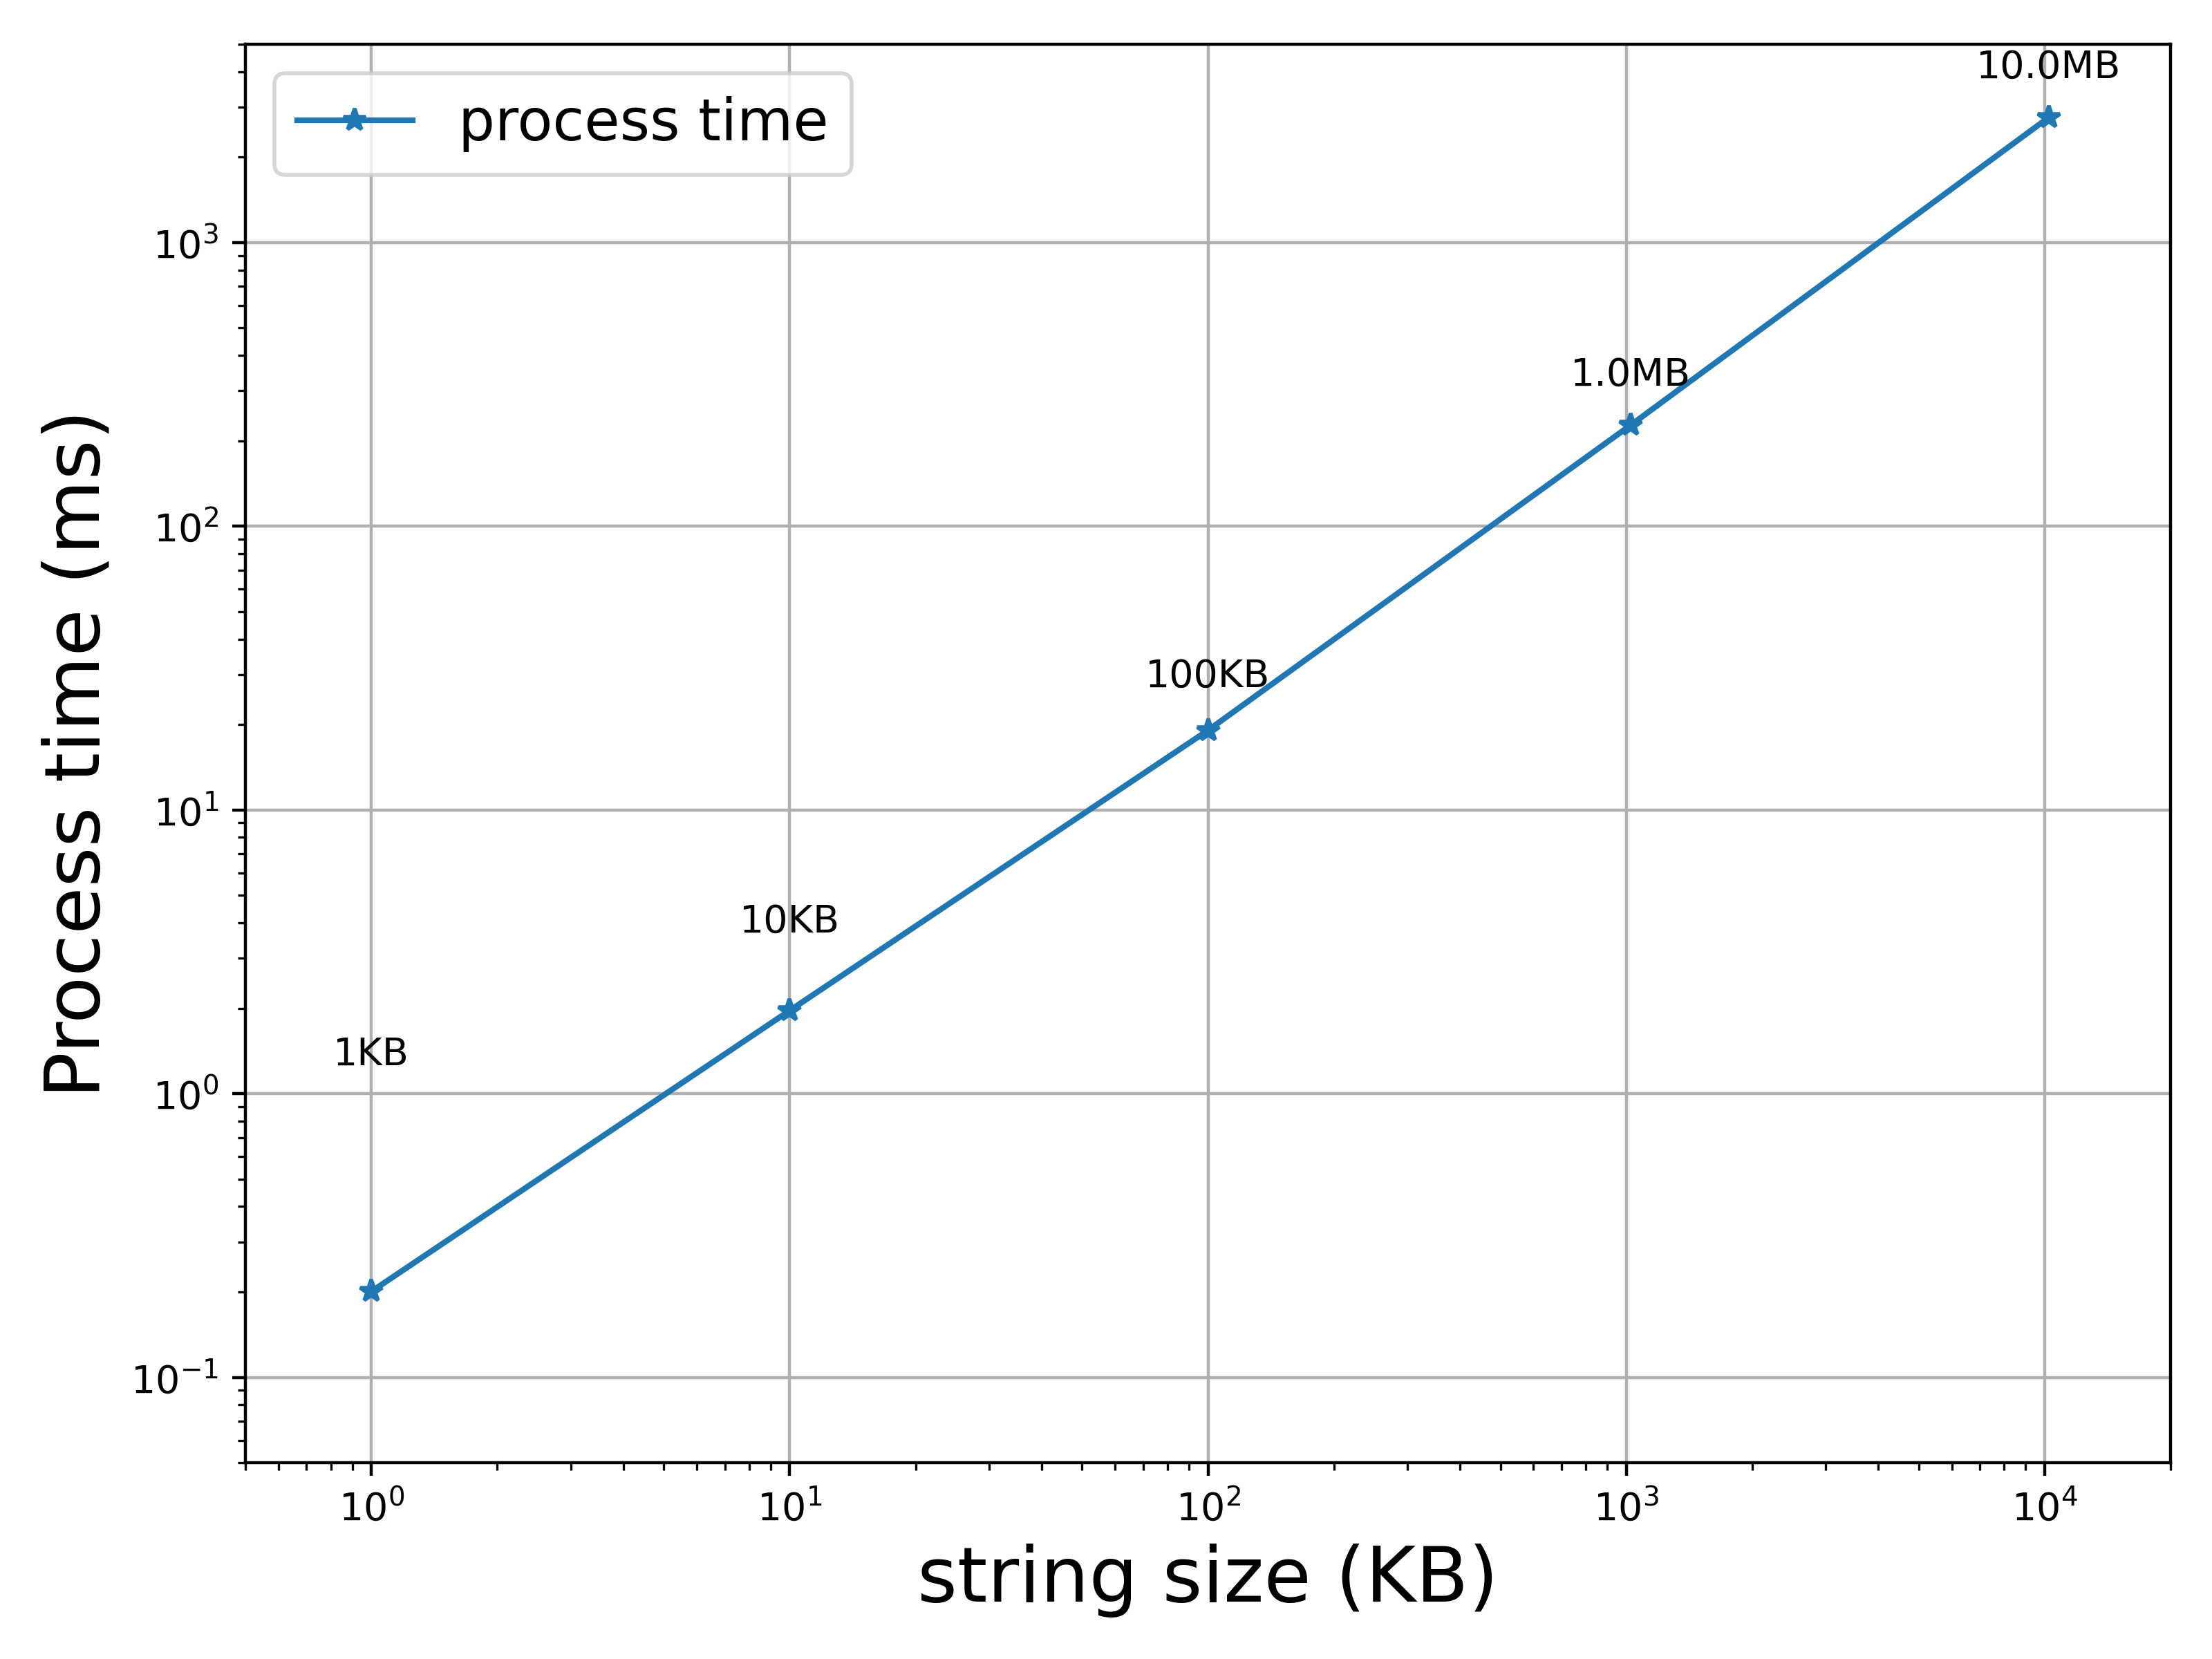
\includegraphics[width=\textwidth]{figures/tests/proportional_tests/Average_string_messages_sending_time_of_100_tests_1KB_to_10MB.png}
        \caption{} \label{fig: proportional-stringsize-a}
    \end{subfigure}
    \begin{subfigure}{0.49\textwidth}
        \centering
        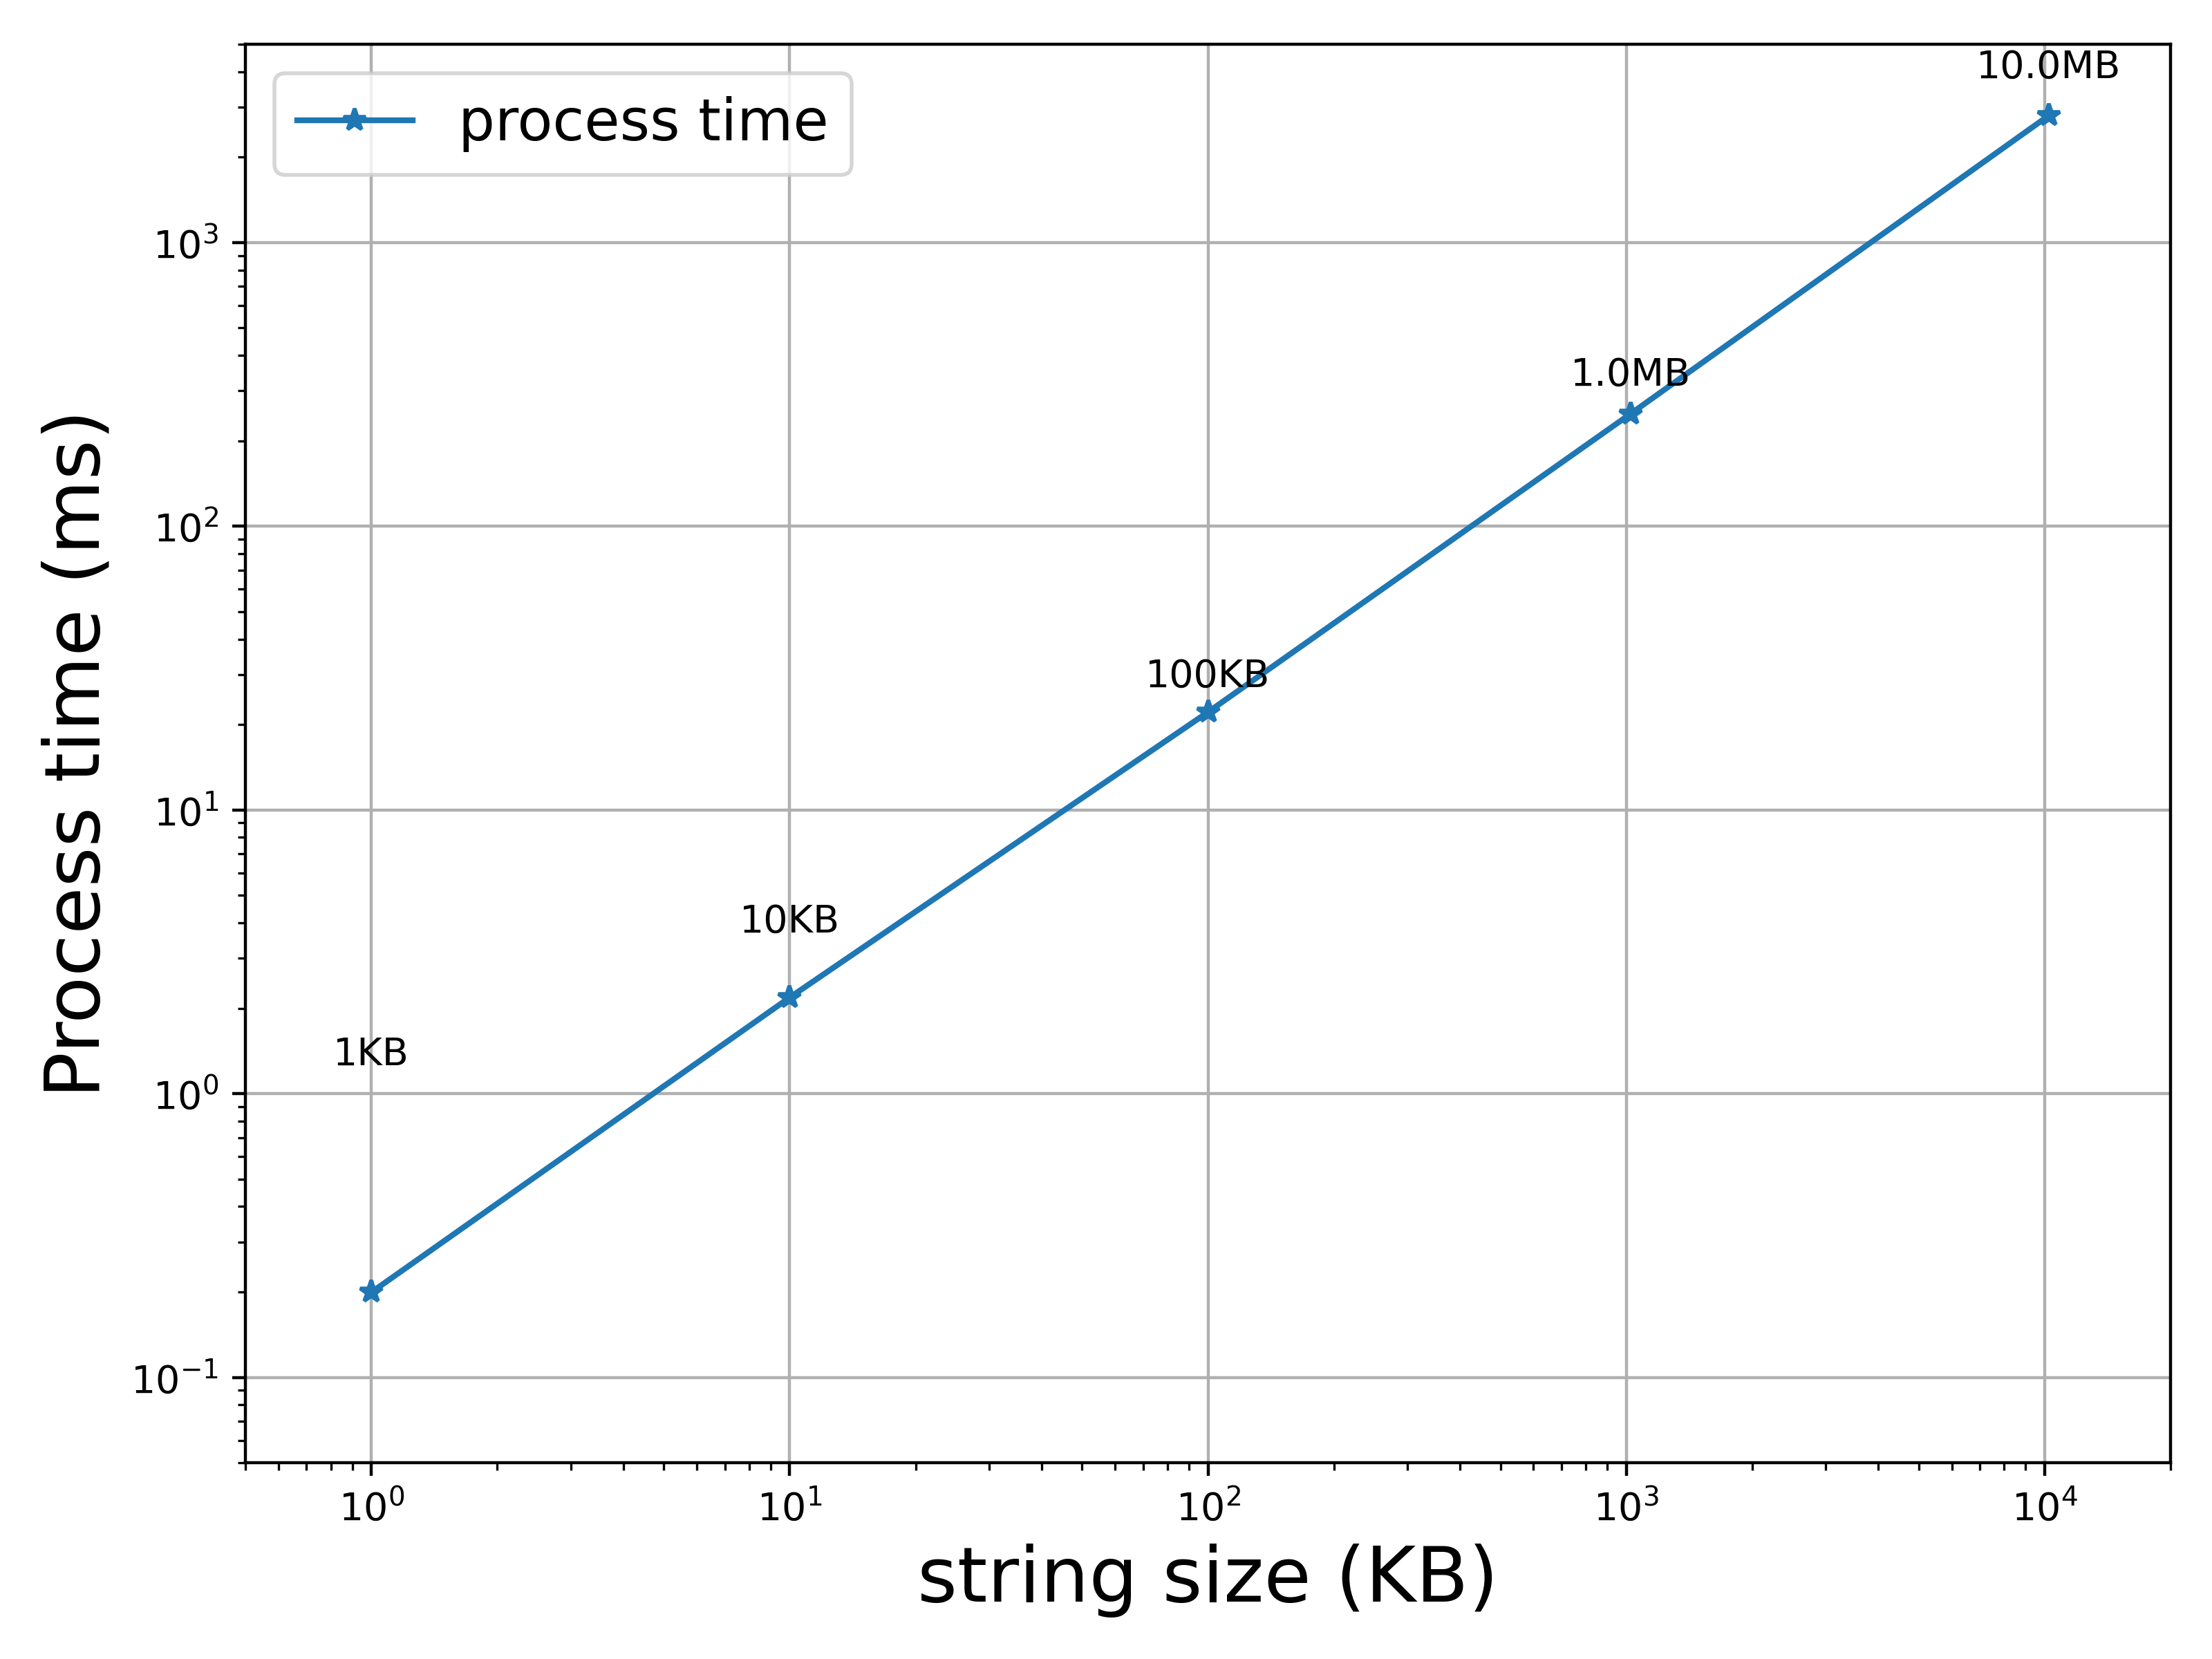
\includegraphics[width=\textwidth]{figures/tests/proportional_tests/Average_string_messages_receiving_time_of_100_tests_1KB_to_10MB.png} 
        \caption{} \label{fig: proportional-stringsize-b}
    \end{subfigure} 

    \caption{Average delay of sending and receiving a string message varied from 1KB 
    to 10MB for 100 times between 2 clients. (\subref{fig: proportional-stringsize-c}) Messages clientS sent forward, 
    (\subref{fig: proportional-stringsize-d}) response messages from clientR, 
    (\subref{fig: proportional-stringsize-a}) process time of massages sent forward 
    and (\subref{fig: proportional-stringsize-b}) process time of massages respond. 
    \label{fig: proportional-stringsize}}
\end{figure}

\subsubsection{Increasing jsonified image message size}
In addition to string, images are also frequently tranported between different agents. 
However, unlike most string messages, image size could be significantly larger 
and even up to over 100MB (raw images). Moreover, the agents ID or message priority 
information should also be included in the message. Therefore, the image should 
be first jsonified with necessary information and then sent to the server. 
The tests for images are done similar to the string message, with an image size 
varies from 1KB to 100MB. 


In fig.\ref{fig: proportional-imagesize-a} and \ref{fig: proportional-imagesize-b} 
again shows the linear dependency of latency and jsonified image size. 
Although the image test results in a 
transmisson time from 1KB to 10MB message length similar to string test, 
there is a huge difference in terms of process time between both. By comparing the 
fig.\ref{fig: proportional-stringsize-c} with \ref{fig: proportional-imagesize-c} 
and fig.\ref{fig: proportional-stringsize-d} with \ref{fig: proportional-imagesize-d}, 
the server process time of string messages is much higher than that for the 
image message. Meanwhile, due to the additional overhead of json format, the network 
delay of string messages is relative smaller than image messages. 


A possible reason for the larger process time for string is that, a string message 
received by server must be processed twice: splitting the message to extract the client 
ID and recombining it for further transport. Meanwhile a jsonified image will only be 
processed once to extract the client information and the original json file will be 
futher transported directly.     
\begin{figure}[htb]
        \centering
    \begin{subfigure}{0.49\textwidth}
        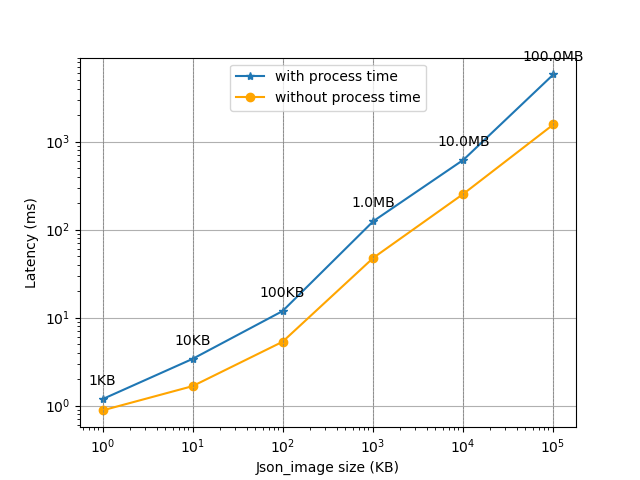
\includegraphics[width=\textwidth]{figures/tests/proportional_tests/log_Average_json_image_messages_sending_time_of_100_tests_1KB_to_100MB.png}\hfill 
        \caption{} \label{fig: proportional-imagesize-c}
    \end{subfigure}
    \begin{subfigure}{0.49\textwidth}
        \centering
        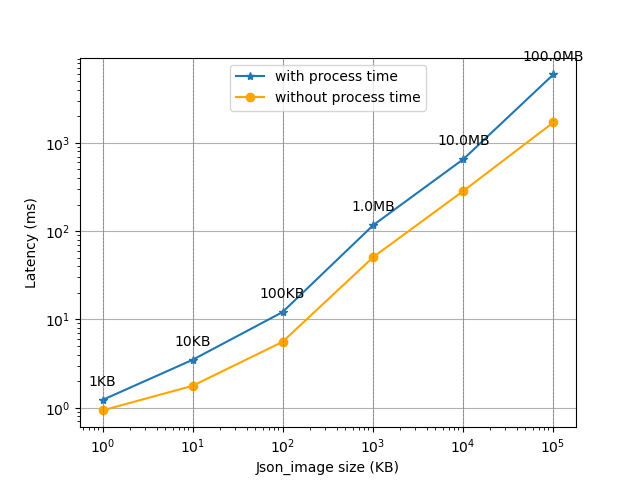
\includegraphics[width=\textwidth]{figures/tests/proportional_tests/log_Average_json_image_messages_receiving_time_of_100_tests_1KB_to_100MB.png}\hfill 
        \caption{} \label{fig: proportional-imagesize-d}
    \end{subfigure}
    \begin{subfigure}{0.49\textwidth}
        \centering
        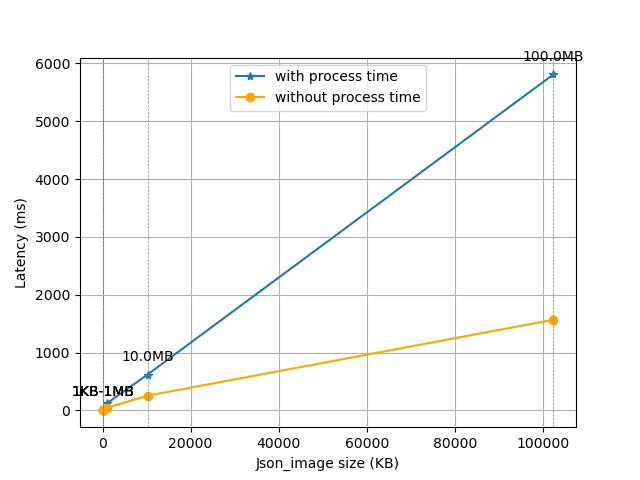
\includegraphics[width=\textwidth]{figures/tests/proportional_tests/Average_json_image_messages_sending_time_of_100_tests_1KB_to_100MB.png}\hfill 
        \caption{} \label{fig: proportional-imagesize-a}
    \end{subfigure}
    \begin{subfigure}{0.49\textwidth}
        \centering
        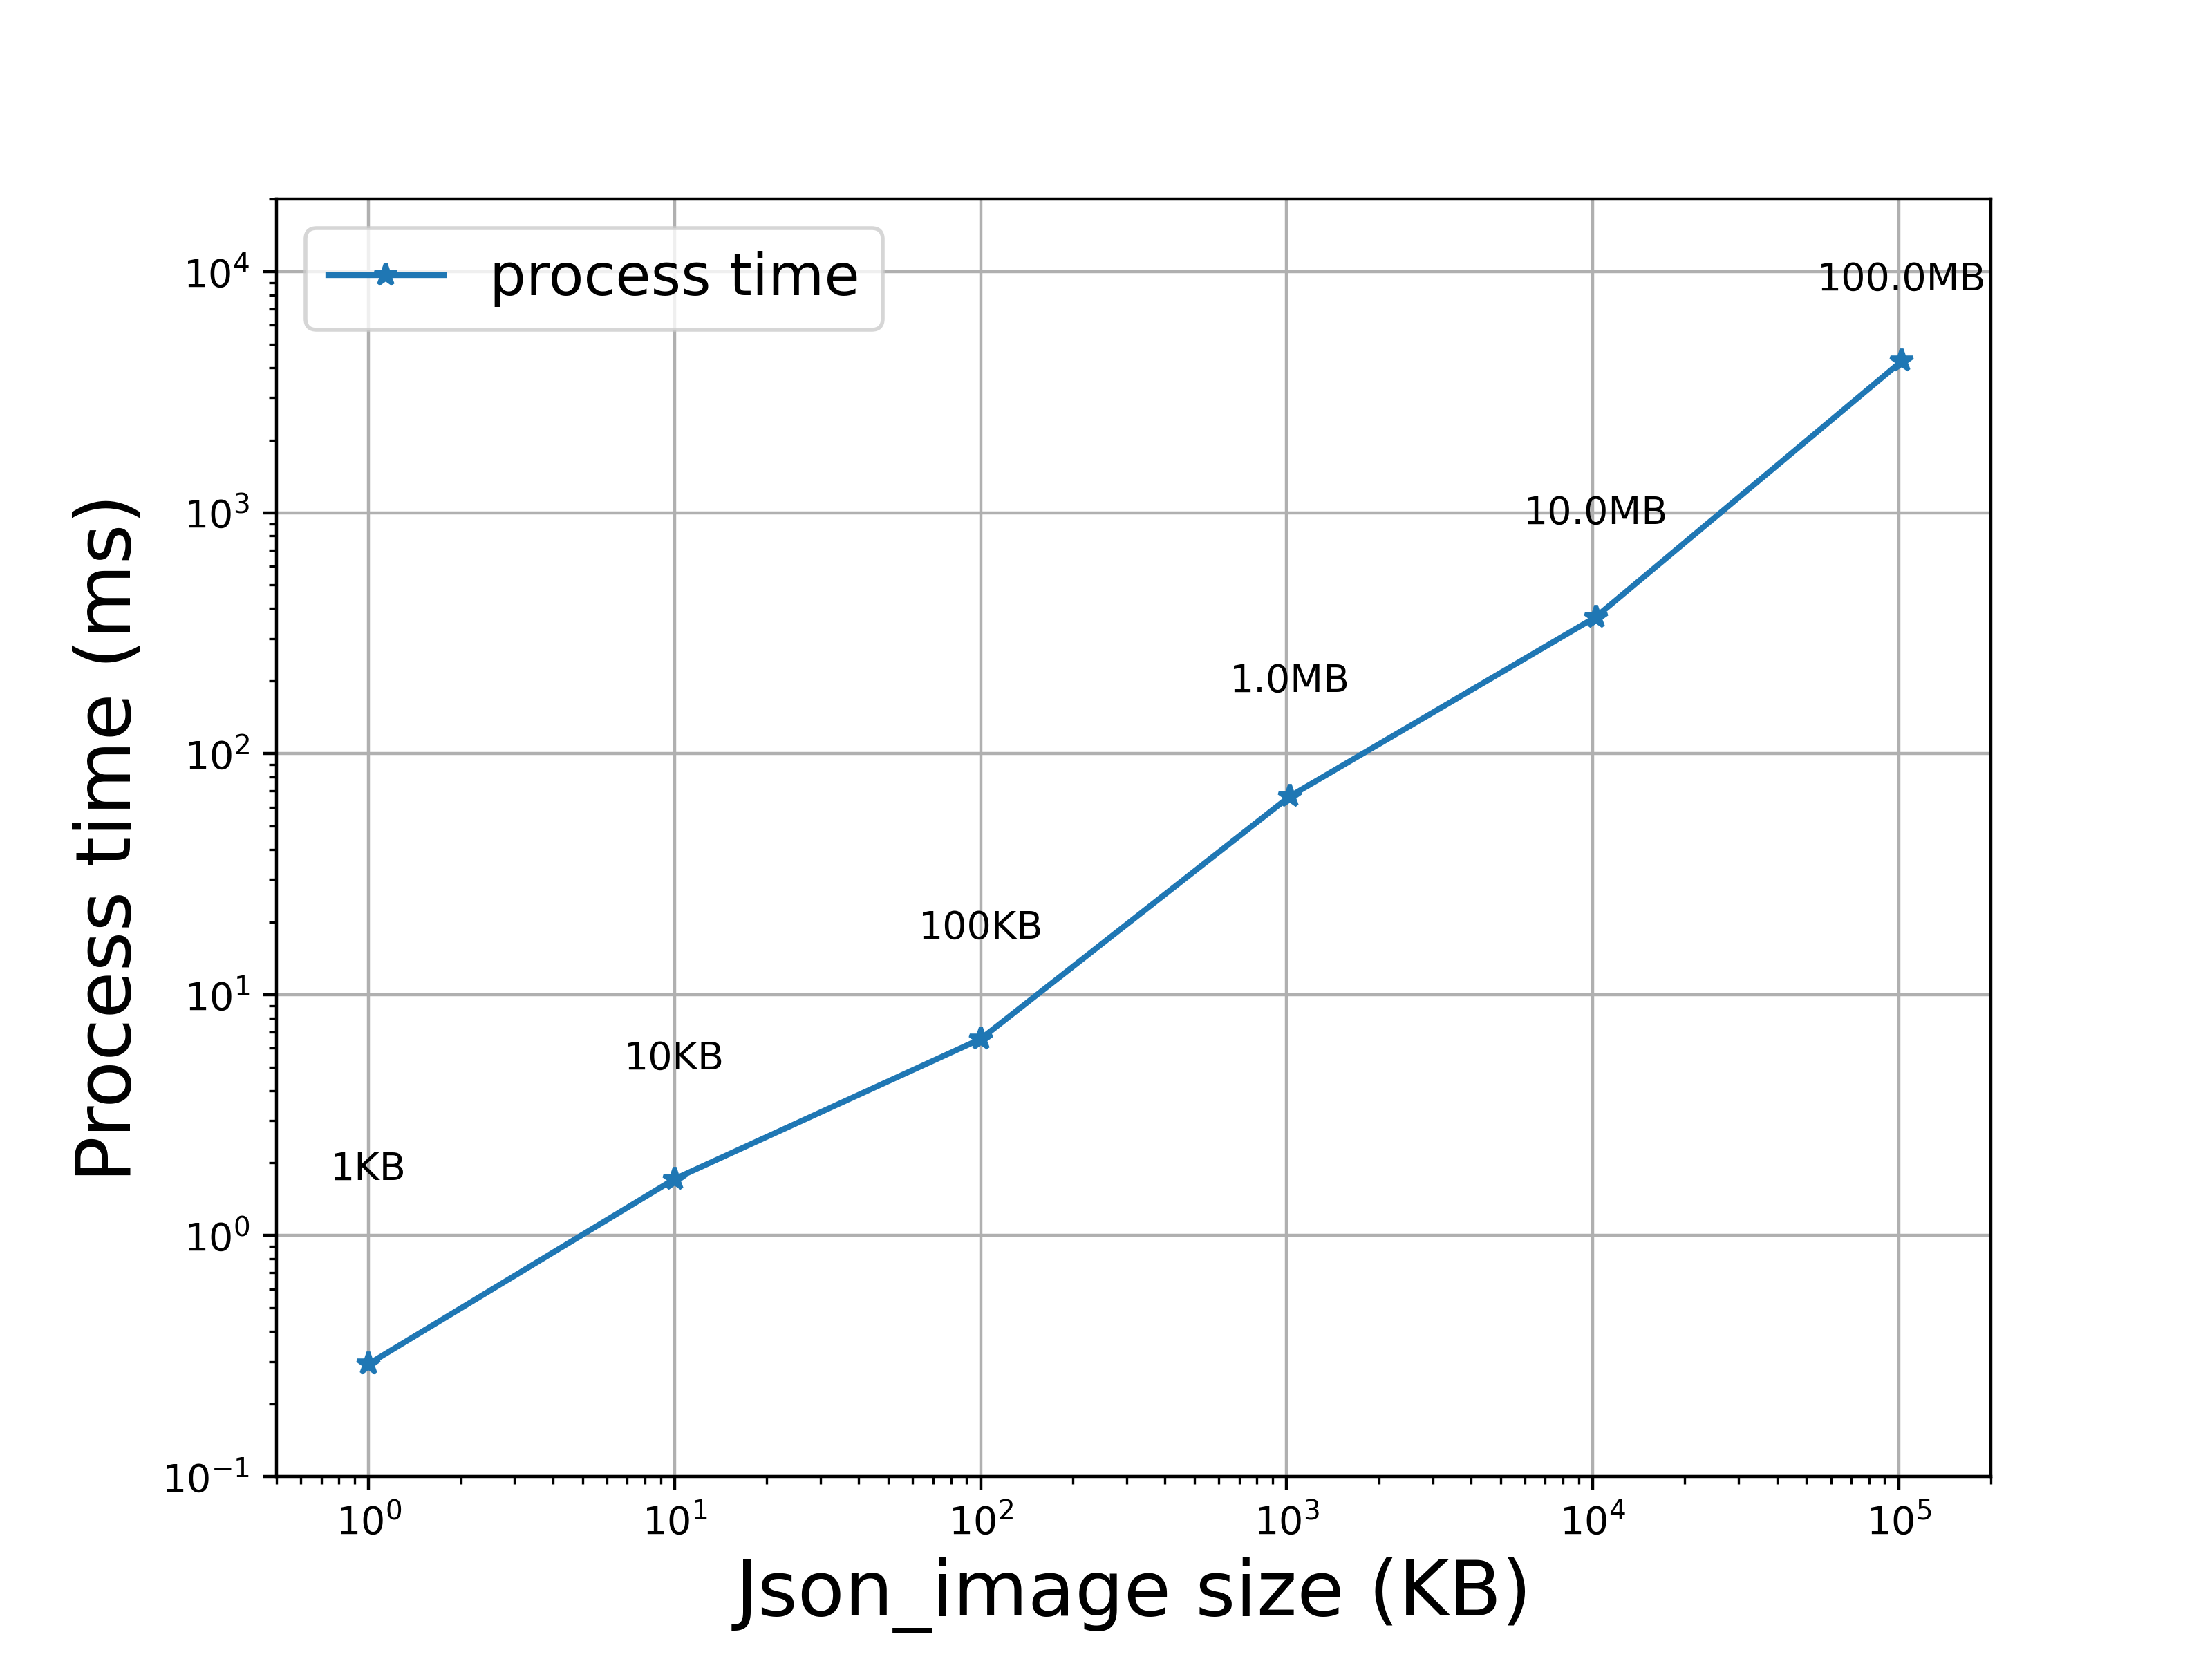
\includegraphics[width=\textwidth]{figures/tests/proportional_tests/Average_json_image_messages_receiving_time_of_100_tests_1KB_to_100MB.png}\hfill 
        \caption{} \label{fig: proportional-imagesize-b}
    \end{subfigure}

    \caption{Average delay of sending and receiving a jsonified image message varied from 1KB 
    to 100MB for 100 times between 2 clients. (\subref{fig: proportional-imagesize-c}) 
    Messages clientS sent forward in log form, 
    (\subref{fig: proportional-imagesize-d}) response messages from clientR in log form, 
    (\subref{fig: proportional-imagesize-a}) process time of messages sent forward  
    and (\subref{fig: proportional-imagesize-b}) process time of response messages from clientR. 
    \label{fig: proportional-imagesize}}
\end{figure}


\subsection{Test results of WebSocket and \gls{http}} \label{chap: Result-RestFUL_WS}
After testing the performance of the WebSocket based communication system, 
it will be interesting to see whether the other application layer protocols with 
different message transport mechanism will have a similar or completely different 
performance under the same conditions. As demonstrated from the 
fig.\ref{fig: MsgConceptual}, \gls{http} is designed for message 
transfer in both directions, and therefore more comparable with WebSocket among the others. 
A common interface for web service design based on \gls{http} is called RESTful API, 
which supports more features than common \gls{http} API. As a result, RESTful API will 
be used for the design of a similar architecture as WebSocket and 
tested under the same condition of the WebSocket string test.


\begin{figure}[htb]
    \begin{subfigure}[b]{0.49\textwidth}
        \centering
        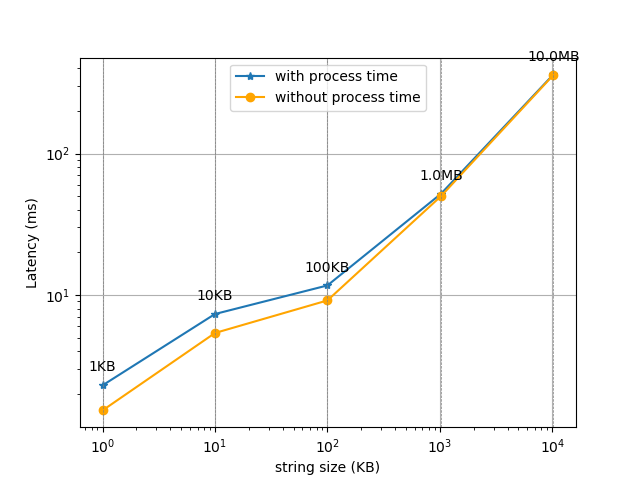
\includegraphics[width=\textwidth]{figures/tests/proportional_tests/Rest_log_Average_string_messages_sending_time_of_100_tests.png}\hfill 
        \caption{} \label{fig: proportional-rest-stringsize-c}
    \end{subfigure}
    \begin{subfigure}[b]{0.49\textwidth}
        \centering
        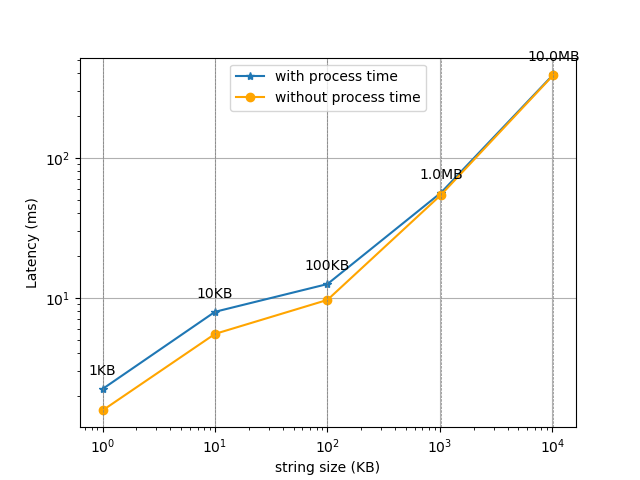
\includegraphics[width=\textwidth]{figures/tests/proportional_tests/Rest_log_Average_string_messages_receiving_time_of_100_tests.png}\hfill 
        \caption{} \label{fig: proportional-rest-stringsize-d}
    \end{subfigure}

    \begin{subfigure}[b]{0.49\textwidth}
        \centering
        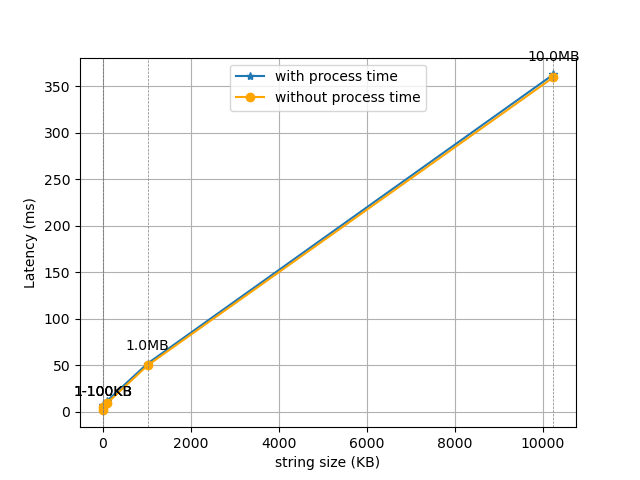
\includegraphics[width=\textwidth]{figures/tests/proportional_tests/Rest_Average_string_messages_sending_time_of_100_tests.png}\hfill 
        \caption{} \label{fig: proportional-rest-stringsize-a}
    \end{subfigure}
    \begin{subfigure}[b]{0.49\textwidth}
        \centering
        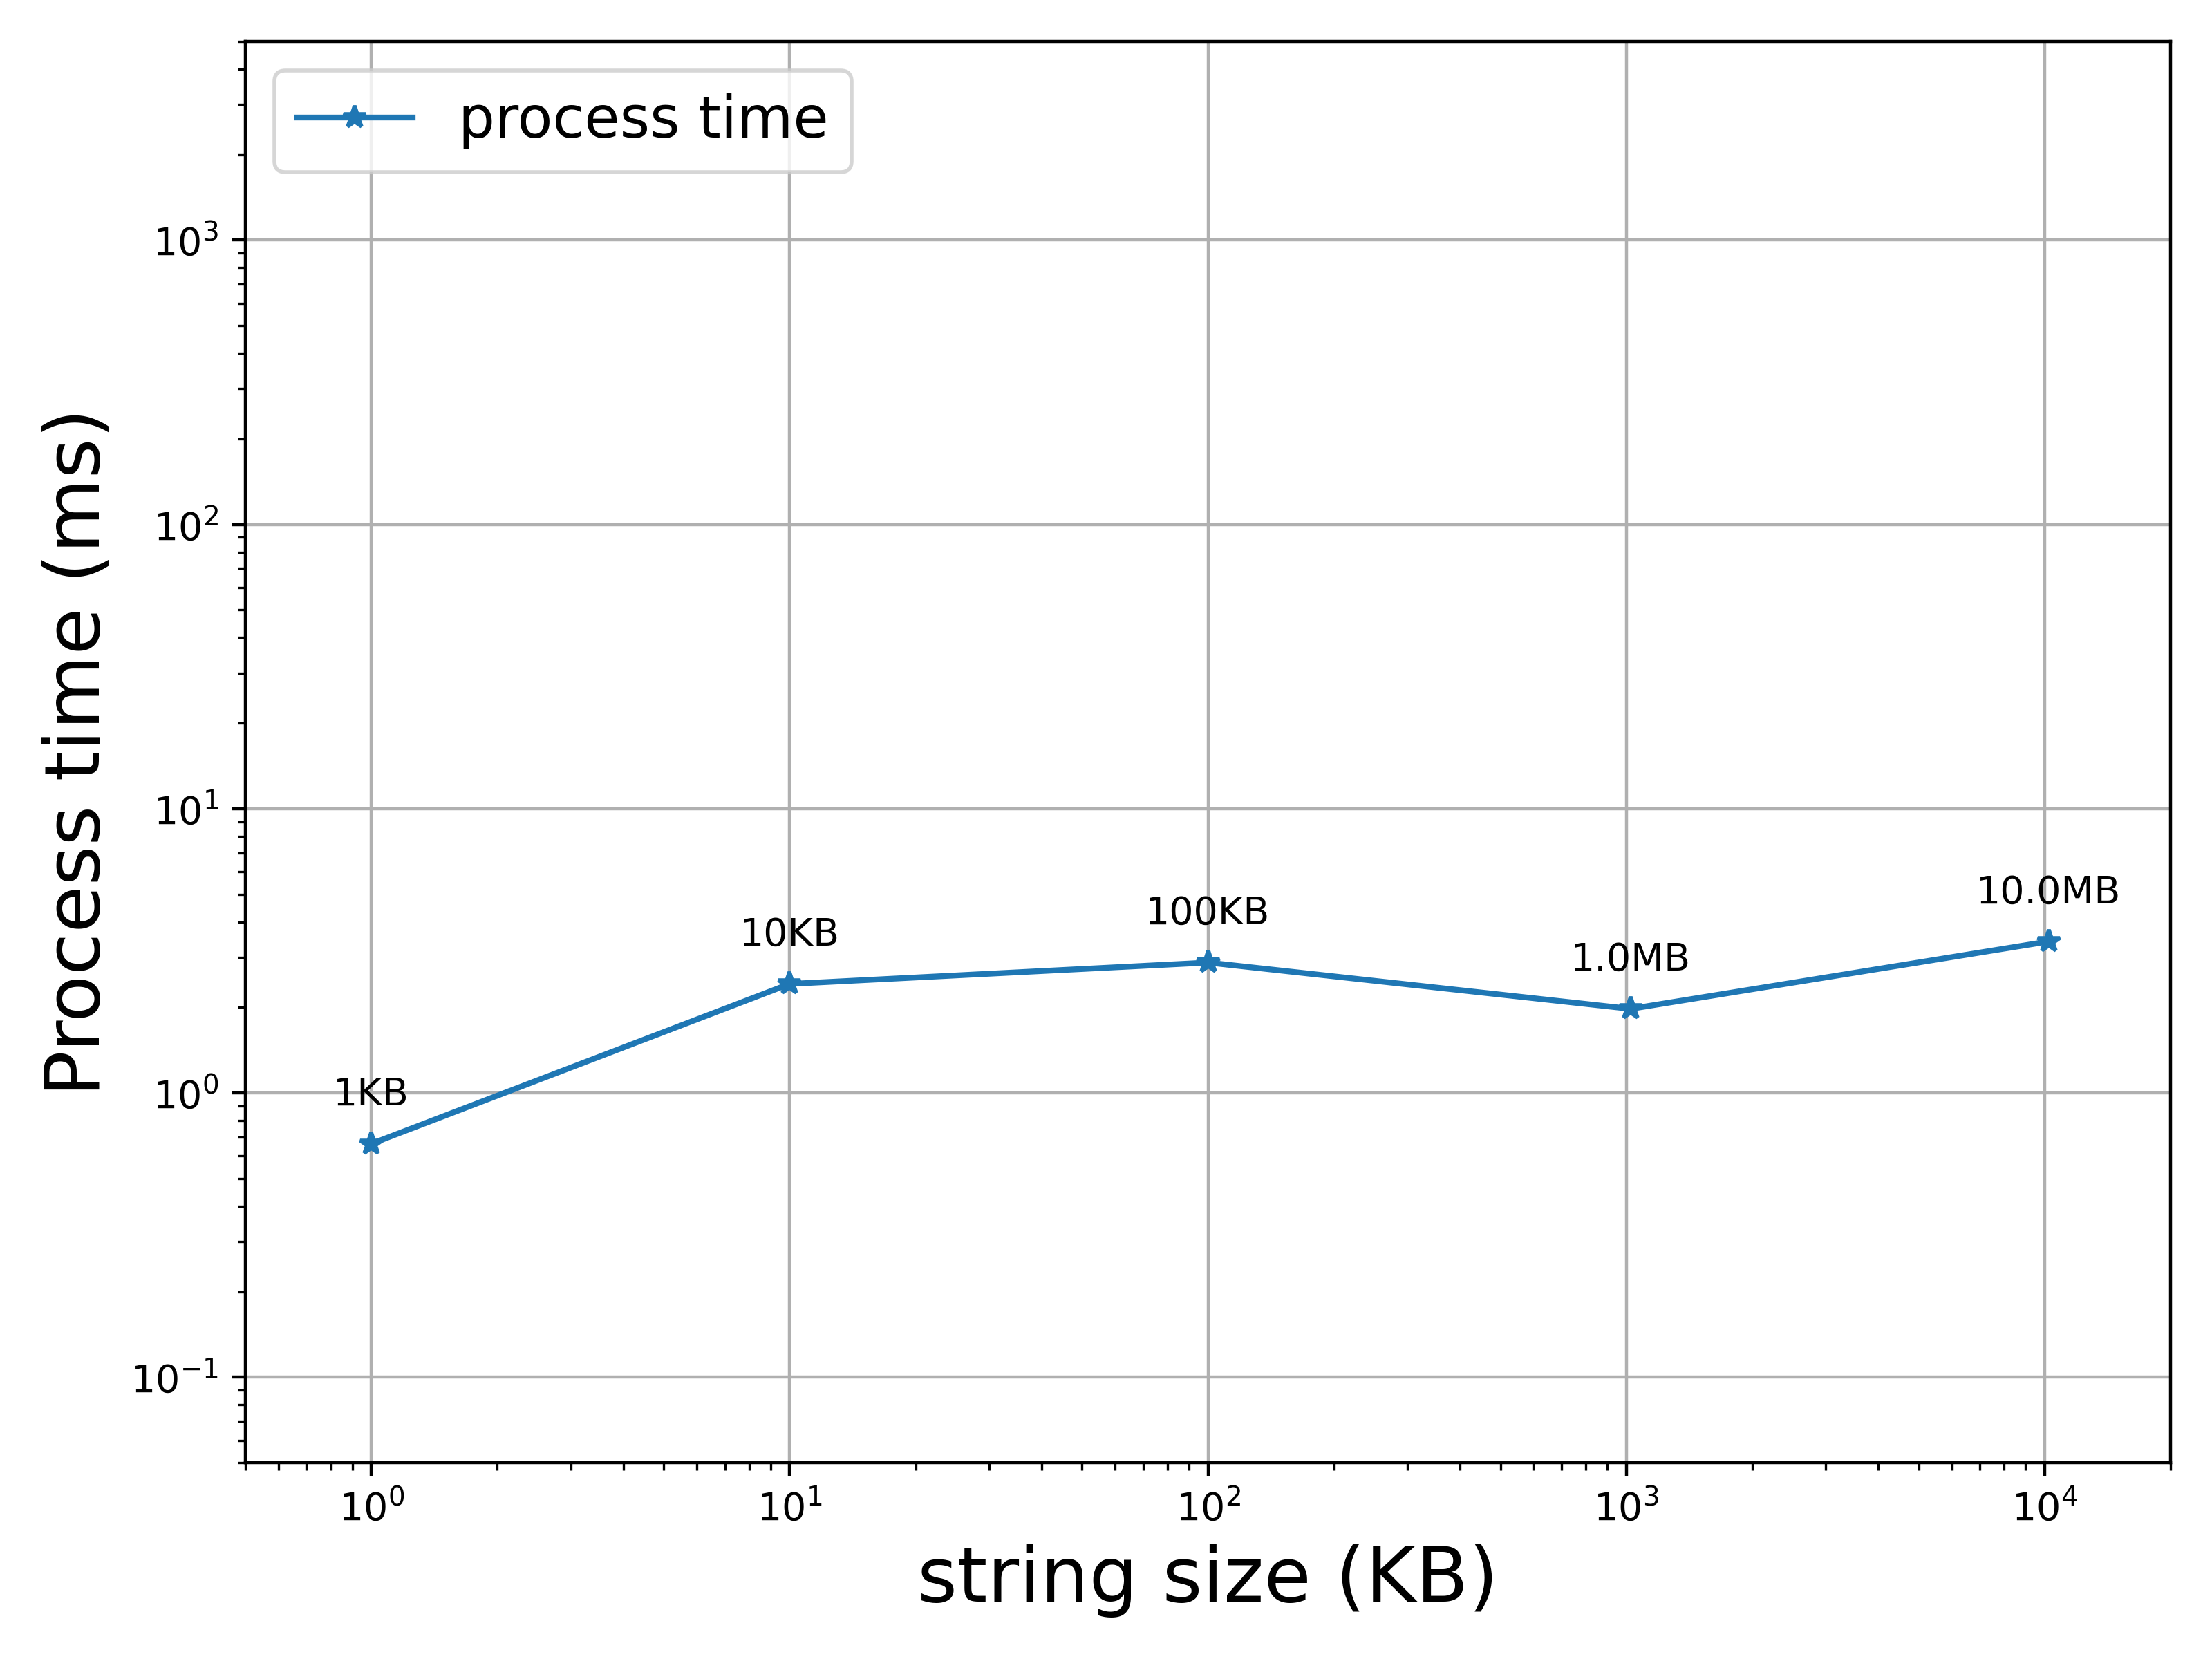
\includegraphics[width=\textwidth]{figures/tests/proportional_tests/Rest_Average_string_messages_receiving_time_of_100_tests.png}\hfill 
        \caption{} \label{fig: proportional-rest-stringsize-b}
    \end{subfigure}
    
    \caption{RESTful API: Average delay of sending and receiving a string message varied from 1KB 
    to 10MB for 100 times between 2 clients. (\subref{fig: proportional-rest-stringsize-c}) 
    Messages clientS sent forward, 
    (\subref{fig: proportional-rest-stringsize-d}) response messages from clientR, 
    (\subref{fig: proportional-rest-stringsize-a}) process time of messages sent forward 
    and (\subref{fig: proportional-rest-stringsize-b}) process time of messages respond. 
    \label{fig: proportional-rest-stringsize}}
\end{figure}

\subsection{priority tests of WS server in diff. performance testing} \label{chap: Result-priority}

\section{External}\label{chap: Result-External}

\subsection{Test results of DTagents related to Azure Digital Twin} \label{chap: Result-DT}